\documentclass[a4paper]{article}
\usepackage[spanish]{babel}
\usepackage[utf8]{inputenc}
\usepackage{fancyhdr}
%\usepackage{charter}   % tipografía
\usepackage{graphicx}
\usepackage{makeidx}
\usepackage{mathptmx}

\usepackage{float}
\usepackage{amsmath, amsthm, amssymb}
\usepackage{amsfonts}
\usepackage{sectsty}
\usepackage{wrapfig}
\usepackage{listings} % necesario para el resaltado de sintaxis
\usepackage{caption}
%%%%%%%%%% Paquete para hacer grafos
%%% ver link http://www.texample.net/tikz/examples/bridges-of-konigsberg/
%\usepackage{fullpage}
%\usepackage{fourier}
\usepackage{tikz}
\usetikzlibrary{arrows,%
                shapes,positioning}
                
\thispagestyle{empty}
%%%%%%%%%% Fin paquete para hacer grafos
%%%%%%%%%%
\usepackage{hyperref} % agrega hipervínculos en cada entrada del índice
\hypersetup{          % (en el pdf)
    colorlinks=true,
    linktoc=all,
    citecolor=black,
    filecolor=black,
    linkcolor=black,
    urlcolor=black
}

\usepackage{color} % para snippets de código coloreados
\usepackage{fancybox}  % para el sbox de los snippets de código

\definecolor{litegrey}{gray}{0.94}

% \newenvironment{sidebar}{%
% 	\begin{Sbox}\begin{minipage}{.85\textwidth}}%
% 	{\end{minipage}\end{Sbox}%
% 		\begin{center}\setlength{\fboxsep}{6pt}%
% 		\shadowbox{\TheSbox}\end{center}}
% \newenvironment{warning}{%
% 	\begin{Sbox}\begin{minipage}{.85\textwidth}\sffamily\lite\small\RaggedRight}%
% 	{\end{minipage}\end{Sbox}%
% 		\begin{center}\setlength{\fboxsep}{6pt}%
% 		\colorbox{litegrey}{\TheSbox}\end{center}}

\newenvironment{codesnippet}{%
	\begin{Sbox}\begin{minipage}{\textwidth}\sffamily\small}%
	{\end{minipage}\end{Sbox}%
		\begin{center}%
		\colorbox{litegrey}{\TheSbox}\end{center}}



\usepackage{fancyhdr}
\pagestyle{fancy}

%\renewcommand{\chaptermark}[1]{\markboth{#1}{}}
\renewcommand{\sectionmark}[1]{\markright{\thesection\ - #1}}

\fancyhf{}

\fancyhead[LO]{Sección \rightmark} % \thesection\
\fancyfoot[LO]{\small{Camila Coy, Uriel Fadel, Jorge Porto, Carlos Soliz}}
\fancyfoot[RO]{\thepage}
\renewcommand{\headrulewidth}{0.5pt}
\renewcommand{\footrulewidth}{0.5pt}
\setlength{\hoffset}{-0.8in}
\setlength{\textwidth}{16cm}
%\setlength{\hoffset}{-1.1cm}
%\setlength{\textwidth}{16cm}
\setlength{\headsep}{0.5cm}
\setlength{\textheight}{25cm}
\setlength{\voffset}{-0.7in}
\setlength{\headwidth}{\textwidth}
\setlength{\headheight}{13.1pt}

\renewcommand{\baselinestretch}{1.1}  % line spacing


\usepackage{underscore}
\usepackage{caratula}
\usepackage{url}
\usepackage{color}
\usepackage{clrscode3e} % necesario para el pseudocodigo (estilo Cormen)

%\usepackage{algorithm}
%\usepackage{algorithmic}
\usepackage{algorithm}[1]
\usepackage{algorithmic}[1]
%\usepackage{algpseudocode}

\definecolor{dkgreen}{rgb}{0,0.6,0}
\definecolor{gray}{rgb}{0.5,0.5,0.5}
\definecolor{mauve}{rgb}{0.58,0,0.82}

\definecolor{gray}{gray}{0.5}
\definecolor{light-gray}{gray}{1}
\definecolor{orange}{rgb}{1,0.5,0}

\lstset{frame=tb,
  language=JAVA,
  aboveskip=3mm,
  belowskip=3mm,
  showstringspaces=false,
  columns=flexible,
  basicstyle={\small\ttfamily},
  keywordstyle=\color{blue},
  commentstyle=\color{dkgreen},
  stringstyle=\color{mauve},
  breaklines=true,
  breakatwhitespace=true,
  tabsize=3,
  numbers=left,
  xleftmargin=2em,
  frame=single,
  framexleftmargin=2em,
  numbersep=5pt,                   % how far the line-numbers are from the code
  numberstyle=\small\color{gray} % the style that is used for the line-numbers
 }
 
 \lstdefinestyle{customc}{
  backgroundcolor=\color{light-gray},
  belowcaptionskip=1\baselineskip,
  breaklines=true,
  numbers=left,
  xleftmargin=\parindent,
  language=C++,
  showstringspaces=false,
  basicstyle=\footnotesize\ttfamily,
  keywordstyle=\bfseries\color{blue},
  commentstyle=\itshape\color{gray},
  identifierstyle=\color{black},
  stringstyle=\color{orange},
}

\begin{document}


\thispagestyle{empty}
\materia{Algoritmos y estructuras de dato III}
\submateria{Segundo Cuatrimestre de 2015}
\titulo{Diseño de algoritmos sobre grafos}
\subtitulo{Aplicación de técnicas 2.0}
\integrante{Coy, Camila Paula}{33/14}{camicoy94@gmail.com} % por cada integrante (apellido, nombre) (n° libreta) (e-mail)
\integrante{Fadel, Uriel}{104/14}{urielfadel@gmail.com}
\integrante{Porto, Jorge}{376/11}{cuanto.p.p@gmail.com}
\integrante{Soliz, Carlos}{406/12}{rcarlos.cs@gmail.com}

\maketitle
\newpage

\thispagestyle{empty}
\vfill

\thispagestyle{empty}
\vspace{1.5cm}
\tableofcontents
\newpage

%\normalsize

\newpage
\section{Objetivos generales}
\setcounter{page}{1}

El objetivo del siguiente trabajo sera la práctica de distintos técnicas para elaboración de algoritmos.
Tal trabajo consta de tres situaciones que bien pueden ser aplicadas a la vida real, se buscara resolverlos de forma óptima. \newline
En el primer problema se aplicaran algoritmos de programación dinámica. El segundo y tercer problemas, se modelaran en grafos, para así llegar obtener de manera óptimas resultados, esto algoritmos estarán basados en dfs y krukal levemente modificados.  
%\newpage



%\newpage
\section{Problema 1}
\subsection{Descripción del problema.}

\vspace*{0.3cm}



\textbf{Introducción al problema} \newline


\vspace*{0.3cm}

%Estamos en el año 2048 y el pabellon 0+infinito es todo un exito. Los alumnos de algoritmos 3. Los alumnos de algoritmos 3 estan muy contentos porque van a cursar este cuatrimestre en un aula que está en el piso N, que es el más alto de todos. Con los avances de la ciencia y tegnologia, escaleras y ascensores han quedado obsoletos, y la forma de subir de un piso a otro es a través de portales. El nuevo pabellón tiene P portales, cada uno de los cuales permite subir de un piso A a un piso más alto B(para bajar de piso hay que tirarse con un paracaídas al piso 0 y luego volver a subir de ser necesario). 

%Uno de los alumnos, que estaba cursando en el segurno cuatrimestre de 2015 y fue congelado por el método de criogenia, acaba de ser descongelado y no puede creer lo bueno que están estos portales, algo que en su epoca no existía . Luego de completar todos los censos de estudiantes desde el año 2015 en adelate, este alumno quiere usar la mayor cantidad de portales posibles para legar al piso N y así seguir cursando Algoritmos III. Diseñar un algoritmo de complejidad $O(N^2)$ para calcular la mayor cantidad de portales que puede utilizar el alumno para subir desde planta baja al piso N (sin tirarse nunca con paracaídas). Se asegura que en toda instancia del problema es posible realizar el recorrido deseado, y que no hay más de un portal que comunique el mismo para de pisos. 

Estamos ubicados en el año 2048 y el pabellón 0+infinito es todo un éxito. Ese cuatrimestre les toco a los alumnos de algoritmos III cursar en el ultimo piso (piso N) y están muy contentos por eso.\newline
Con el avance de la ciencia y tecnología los ascensores, escaleras han quedado muy antiguos(obsoletos), es su lugar se han usado portales que \underline{sirven solamente para subir} de un piso a otro. \newline 
Este actual pabellón tiene P portales, cada uno de estos permite subir desde un piso A a un piso B, donde piso piso A es menor que el piso B.
La única manera de bajar de un piso es tirándose con paracaídas, el cual llega hasta el piso 0. Por lo cual si nos equivocamos en la elección deberemos intentarlos nuevamente desde el inicio(planta baja).\newline 
Uno de los alumnos, que estaba cursando en el segundo cuatrimestre de 2015, fue congelado por el método de criogenia. Este alumno fue descongelado y esta asombrado por el imponente edificio 0+infinito, y no puede creer lo bueno que están los portales(en su época sólo existían ascensores y escaleras). Luego de cumplir con sus obligaciones de completar los censos de 2015 hasta 2048, este alumno quiere quiere usar la mayor cantidad de portales para llegar al piso N y así llegar a cursar Algoritmos III. \newline

\begin{figure}[H]
  \begin{center}
      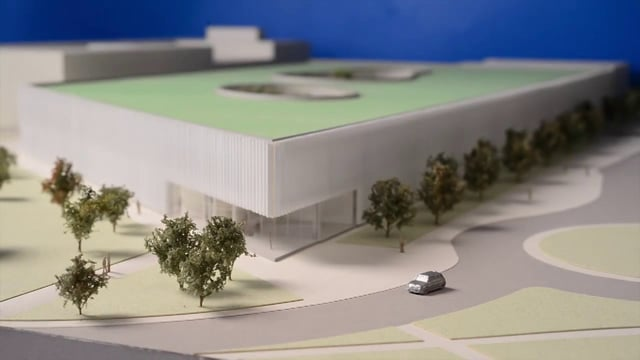
\includegraphics[scale=0.50]{imagenes/cero+infinito2.jpg}
  \end{center}
  \caption{Maqueta de edificio cero+infinito}
\end{figure}

\textbf{Problema a solucionar} \newline

Nuestro objetivo es diseñar un algoritmos de complejidad $O(N^2)$  para calcular la mayor cantidad de portales que puede utilizar este alumno para lograr subir desde planta baja hasta el piso N(no esta de mas decir que alumno no debería tirarse en paracaídas durante el trayecto).
Nos aseguran que en toda instancia del problema se podrá hacer el recorrido deseado y que no hay mas de un portal que comunique el mismo par de pisos.  

%%%%%% Informe anterior mal redactado %%%%

%El siguiente problema que presentaremos bien puede ser una situación que se nos presente en el a corto, mediano o largo plazo en la querida Facultad de Ciencias exacta y naturales. Cómo es sabido desde hace muy poco tiempo, se construirá un edificio el cual sera bautizado con el nombre Pabellón 0+infinito. Este edificio contendrá aulas, bibliotecas, oficinas, etc. Tendrá una cierta cantidad de pisos, que los alumnos, docentes, y otras personas deberán atravesar para llegar a sus respectivos lugares.

%\begin{figure}[H]
%  \begin{center}
%      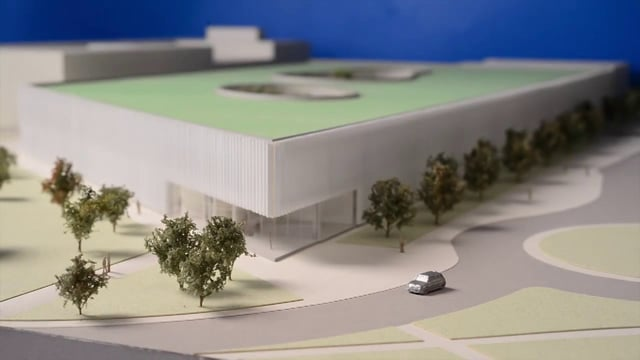
\includegraphics[scale=0.50]{imagenes/cero+infinito2.jpg}
%  \end{center}
%  \caption{Maqueta de edificio cero+infinito}
%\end{figure}



%Un alumno fue congelado por el método de criogenia en el año 2016, ahora es 2048 y este alumno es descongelado.
%El alumno se asombra de que se halla logrado construir el pabellón cero+infinito. Fue tanto su asombro que desea recorrer el edificio antes de ir a cursar algoritmos III. Este edificio cuenta con portales futuristas que comunican dos pisos distintos. 

%\newline
%\textbf{Problema a solucionar: }
%\newline

%El pabellón cero+infinito cuenta con $N$ pisos. 
%El tema es que los pisos están comunicado por $P$ portales, que van de un piso $A$ a otro $B$, dónde el piso $A$ es menor estricto que el piso $B$, osea los portales sólo van de hacia arriba. Y para bajar de los pisos se usan paracaídas que bajan hasta el suelo del pabellón(osea el piso 0), de modo tal que si el estudiante no llega al piso $N$, tendrá que volver a intentarlo. El objetivo del estudiante suba de una sola vez al último piso, atravesando la máxima cantidad de portales posibles. \newline


En los siguientes ejemplos se describirán algunos input del problema que se desea solucionar.
Notar que las columnas indican el piso inicial y final que une el portal, donde piso inicial es la base de la columna y piso final es el tope de la columna. \newline
 
 Ejemplo 1: \newline
 
\begin{figure}[htb]
  \centering
   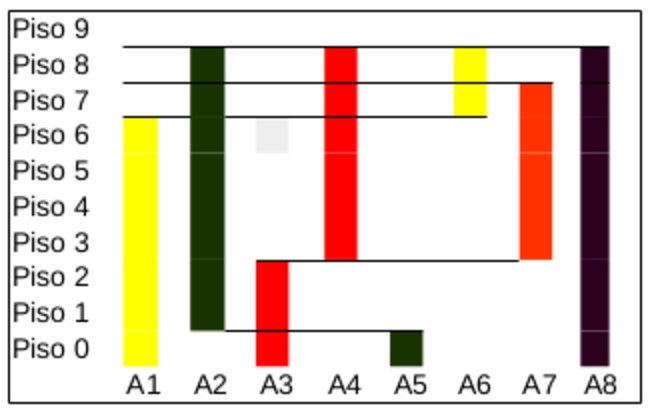
\includegraphics[scale=0.25]{imagenes/problema1Imagen1.jpg}
  \caption{Ejemplo 1}
\end{figure} 



En esta figura tenemos un conjunto de duplas, donde la primer componente de la dupla es el piso inicial, la segunda es el piso llegada: \newline

\begin{itemize}
    \item Input_1: 10 pisos y $\{(0,7),(1,9),(0,3),(3,9),(7,9),(3,8),(0,9)\} $ portales (ver imagen).
    \item Output_1: 2 
\end{itemize}
El output es 2 pues podemos usar dos portales como máximo para llegar al piso nueve(acordarse que siempre arrancamos del piso cero ). Por ejemplo en la figura los portales pueden ser cualquiera de estas tuplas $(A1,A6),(A3,A4)$ ó $(A5,A6)$.
\newline


Ejemplo 2 y 3:


\begin{figure}[H]
   \centering 
      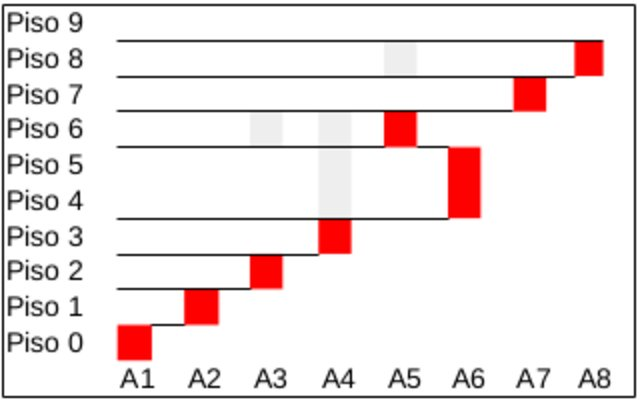
\includegraphics[scale=0.25]{imagenes/problema1Imagen2.jpg}
      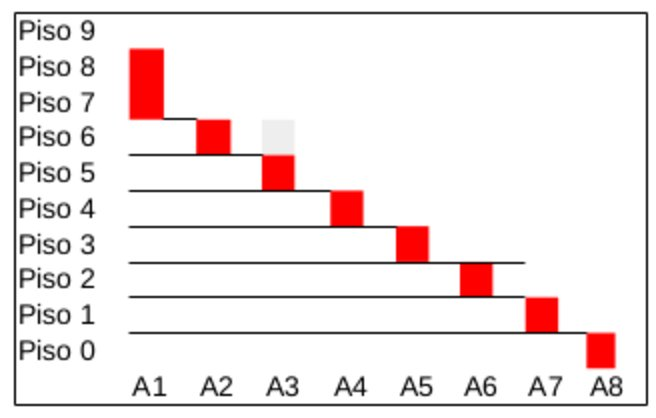
\includegraphics[scale=0.25]{imagenes/problema1Imagen3.jpg}
 \caption{ejemplo 2 y 3}
\end{figure}



\begin{itemize}
    \item Input_2: 10 pisos y $\{(0,1),(1,2),(2,3),(3,4),(6,7),(4,6),(7,8),(8,9)\}$ portales(ver imagen). 
    \item Input_3: 10 pisos y $\{(7,9),(6,7),(5,6),(4,5),(3,4),(2,3),(1,2),(0,1)\}$ portales(ver imagen)
    \item Output_2: 8 , pues debo usar todos los portales. en el siguiente orden \textbf{A1, A2, A3, A4, A6, A5, A7, A8}.  
    \item Output_3: 8 , pues debo usar también todos los portales(mirar figura), en el siguiente orden \textbf{A8, A7, A6, A5, A4, A3, A2, A1}.
\end{itemize}

%	\begin{figure}[htb]
%  \begin{center}
%      \includegraphics[scale=0.25]{imagenes/red-ferroviaria.jpg}
%	  \end{center}
% \caption{ejemplo}
%\end{figure}

\newpage
\subsection{Desarrollo de la idea y pseudocódigo.}

\vspace*{0.3cm}

%\textbf{completar.}
\textbf{}
Para la resolución de este ejercicio nos basamos el la técnica programación dinámica(en nuestro caso usamos bottom up). Lo que hacemos es crear una matriz $M$ de tamaño $nxn$ a la cual llenaremos inicialmente con 0 (ver pseudocódigo linea 2). Sea el elemento contenido en la posición de la  matriz M[i][j], denotamos con i a las filas, y j a las columnas. \newline
Hablemos un poco sobre la matriz y su contenido. Sean $ 0 \leq i \leq j \leq n-1 $: \newline
\begin{itemize}
	\item Solo usaremos la diagonal superior de la matriz.
	\item Si $ M[i][j] = 0 $ quiere decir que no hay forma de llegar él desde el piso $i$ al piso $j$.% pero no que no hay forma de llegar a él tomando mas de un portal.
	\item Si $ M[i][j] = 1 $ quiere decir que existe un portal que va del piso $i$ al piso $j$
	\item Por restricciones del problema se sabe que no exiten portales que unan piso $i$ con piso $i$, osea inicialmente todo $M[i][i] = 0$.  Eventualmente va a cambiar, para todo $i > 0$, y su contenido va a terminar siendo, la maxima cantidad de portales que se puede tomar para llegar a ese piso $i$, desde el primer piso.
%	\item Dentro de la matriz también guardaremos el máximo obtenido hasta el momento preferentemente en  la posición M[i][i] con $0 \leq i \leq n-1 $.
\end{itemize}

Luego recorreremos los portales, y para cada portal P, que va desde el piso $i$ al piso $j$, con $i < j$, se le pondrá en la matriz, en la posición $i,j$ un 1 (Ver linea 6 a 10 del pseudocódigo). \newline
Luego iremos recorriendo la matriz, por su diagonal, ya que ahí es donde guardaremos la máxima cantidad de portales que se puede tomar un alumno  desde el piso $1$ hacia el piso de esa fila. Como vamos avanzamos en la diagonal quiere decir que ya se sabe cuántos portales se puede tomar una persona para llegar a ese piso (no solo sabemos cuánto es sino que está en la diagonal $M[i][j]$, con $i = j$). \newline

Cada iteración vamos a empezar desde la siguiente diagonal (Ver linea 12), y se va a tomar al máximo de esa columna (desde el elemento j = k e i =1,2,..,k -1, hasta la diagonal “k”, sin incluir) como se muestra en el pseudocódigo lineas 16 a 19. Este valor es el que se va a guardar en la diagonal(ver linea 21), y luego en toda la fila de la diagonal, van a estar los portales que salen desde ese piso, ya que como sabemos todo elemento de la matriz que está a la derecha mío todavía no fue recorrido. Asi que tienen un 1, si desde ese piso i, puede llegar al piso j, o un 0 si no se puede llegar.

Entonces al sumarle la maxima cantidad de portales que se pueden tomar para llegar a ese piso, quedara actualizada la cantidad de portales que se puede tomar para llegar al piso $j$, desde el primer piso, habiendo tomado el piso $i$. En el caso en que la diagonal tenga un cero claramente no se puede acceder, vamos a poner a todos los elementos de la derecha de su fila un 0 (ya que desde ese piso no son accesibles).
Dejando a ese piso, con las distancias correctas, y con distancias me refiero a la cantidad de portales para llegar a ese piso desde el piso 1. \newline

Luego finalmente al llegar al final de la matriz(osea $ M[n-1][n-1] $), en ese lugar obtendremos la máxima cantidad de portales que se pueden utilizar para llegar desde el piso 1 hacia el piso n (Ver linea 30). \newline


%%%% expliacion de resolucion del problema que poco claro %%%%

%La resolución de este ejercicio está basado en programación dinámica(bottom up). Lo que hacemos es crear una matriz $M$ de tamaño $NxN$. Sea el elemento contenido en la pisiciond de la  matriz M[i][j], denotamos con i a las filas, y j a las columnas. \newline
%La matriz inicialmente se va a llenar con 0, cuando desde el piso i no puede ir hasta el piso j. Esto quiere decir que en ese piso no hay un portal que pueda llegar a tal piso, no que no hay forma de llegar a él tomando más de 1 portal. Luego iremos recorriendo la matriz, por su diagonal, ya que ahí es donde guardaremos la máxima cantidad de portales que se puede tomar una persona desde el piso uno hacia el piso de esa fila. Como vamos avanzamos en la diagonal quiere decir que ya se sabe cuántos portales se puede tomar una persona para llegar a ese piso (no solo sabemos cuánto es sino que está en la diagonal M[i][j], con i =j, ya que es la diagonal). Cada iteración vamos a empezar desde la siguiente diagonal, y se va a tomar al máximo de esa columna (desde el elemento j = k e i =1,2,..,k -1, hasta la diagonal “k”, sin incluir) y este valor es el que se va a guardar en la diagonal, y luego en toda la fila de la diagonal, van a estar los portales que salen desde ese piso, ya que como sabemos todo elemento de la matriz que está a la derecha mío todavía no fue recorrido, así que tiene un 1 en los portales y un 0 si no hay portal hacia ese piso. Entonces vamos a sumarle a todos los elementos de mi derecha (de mi fila) que no tengan un cero, lo que quiere decir que podemos acceder a ese piso desde el que estamos, y le vamos a sumar el valor de la diagonal, que es la cantidad máxima de portales que podemos llegar a utilizar para llegar a ese piso, siempre y cuando el elemento de la diagonal es mayor a 0, ya que si es cero quiere decir que no se puede acceder, y si no se puede acceder, vamos a poner a todos los elementos de la derecha de su fila, un 0, ya que desde ese piso no son accesibles, ya que a ese piso como tiene un cero en su diagonal no puede accederse.  Dejando a ese piso, con las distancias correctas, y con distancias me refiero a la cantidad de portales para llegar a ese piso desde el piso 1. \newline
%Luego finalmente al llegar al final de la matriz, (la parte de abajo, de la última columna), en ese lugar obtendremos la máxima cantidad de portales que se pueden utilizar para llegar desde el piso 1 hacia el piso n. \newline

%%% Fin de codigo de explicacion de problema que estaba poco claro %%%


 


\textbf{pseudocodigo} %\newline 

\begin{codebox}
\Procname{$\proc{solve}( n \ int,vector<Portal> \& portales)	$}
	\li \Comment Cada portal tiene dos atributos: pisoDesde y pisoHasta
	\li inicializamos la variable $matriz$ de tamaño $n x n$ con el contenido de todas las posiciones en cero. // $O(n)$
	\li Inicializo variables naturales $pisoD$, $pisoH$, $max$ en 0;
	\li Incializo la variable $portal$ $p$;
	\li \Comment Ingresamos todos los portales a la matriz, idicando con 1 si ese portal comunica esos dos pisos
	\li \For $i \gets 0$ \To $portales.size$ \Do	
	\li 	p = portales[i]
	\li		$pisoD$ = p.pisoDesde
	\li		$pisoH$ = p.pisoHasta
	\li		$matriz[pisoD-1][pisoH-1] \leftarrow  1 $
		\End
	\li \Comment Aca vamos a empezar a recorrer de forma diagonal a la $matriz$ 
	\li \For $i \gets 1 $ \To $ i<n $ \Do 
	\li 	\li \Comment Este for itera $n$ veces, lo de adentro del $for$ es del orden: $O(n-i+i) \Rightarrow O(n)$. Conclusion todo tiene orden $O(n*n)$
	\li		$max \leftarrow 0$
	\li		\For $k \gets 0 $ \To $ k<i $ \Do
	\li			\Comment Este for itera $i$ veces, y lo de adentro es del orden de $O(1)$ $\Rightarrow$ tarda $O(i)$
	\li			\If $ matriz[k][i] > max$
	\li				\Then $max \leftarrow matriz[k][i]$ 
				\End
			\End
	\li		\Comment Tenemos el maximo de la columna, lo que quiere decir que es lo que tardamos en llegar hasta el piso actual.
	\li		$ matriz[i][i] \leftarrow max $		
	\li		\Comment Este for va a iterar n-i veces y lo de adentro lo hace en $O(1)$ $=>$ tarda $O(n-i)$	
	\li		\For $ j \gets i+1 $ \To $ j<n$ \Do  
	\li 		\Comment Este for va a itera $n-i$ veces y lo de adentro se hace en $O(1)$ $\Rightarrow$ $tarda O(n-i)$
	\li 		\If $ max == 0$
	\li 			\Then $ matriz[i][j] \leftarrow 0$
	\li				\Else \Comment Sumamos lo que tardo en llegar a piso actual, si es que ese piso (m [i][j] es accesible, osea tiene un 1)
	\li					\If $matriz[i][j] \neq 0$ 
	\li						\Then $ matriz[i][j] \leftarrow max+1$
						\End
				\End
			\End
		\End 
	\li \Return $matriz[n-1][n-1]$ // retorno la maxima cantidad de portales que se puedieron atravesar hasta el piso_n									      
\end{codebox}

\newpage
\subsection{Justificación de la resolución y demostración de correctitud.}

\vspace*{0.3cm}


La forma de ver  que la solución es correcta, es asumir inicialmente que todos lo portales ya ''están puestos''. Con esto queremos decir que en cada posición $i,j$ de la matriz está un 1 si se puede llegar del piso i al piso j hay un cero si no hay portal que comunique esos pisos. Podemos ver mas formalmente en el gráfico de abajo $0 \leq i < j \leq n-1 $ pueden haber un cero ó 1, y para los elementos de la diagonal para bajo asumimos que todo esta en cero(Ver dibujo abajo).

\begin{equation*}
\begin{bmatrix}
a_{00} & a_{01} & a_{02} & ...... & a_{0k} & ...... & a_{0(n-1)} \\
a_{10} & a_{11} & a_{12} & ...... & a_{1k} & ...... & a_{1(n-1)} \\
a_{20} & a_{21} & a_{22} & ...... & a_{2k} & ...... & a_{2(n-1)} \\
...... & ...... & ...... & ...... & ...... & ...... & ......   \\
a_{k0} & a_{k1} & a_{k2} & ...... & a_{kk} & ...... & a_{k(n-1)} \\
...... & ...... & ...... & ...... & ...... & ...... & ...... \\
%a_{(n-1)1} & a_{(n-1)2} & a_{(n-1)3} & ...... & a_{(n-1)k} & ...... & a_{(n-1)(n-1)} & a_{(n-1)n}\\
a_{(n-1)1} & a_{(n-1)2} & a_{(n-1)3} & ...... & a_{(n-1)k} & ...... & a_{(n-1)(n-1)}
\end{bmatrix}
	\Rightarrow
\begin{bmatrix}
a_{00} & a_{01} & a_{02} & ...... & a_{0k} & ...... & a_{0(n-1)} \\
0      & a_{11} & a_{12} & ...... & a_{1k} & ...... & a_{1(n-1)} \\
0      & 0      & a_{22} & ...... & a_{2k} & ...... & a_{2(n-1)} \\
...... & ...... & ...... & ...... & ...... & ...... & ......   \\
0      & 0      & 0      & ...... & a_{kk} & ...... & a_{k(n-1)} \\
...... & ...... & ...... & ...... & ...... & ...... & ......\\
%a_{(n-1)1} & a_{(n-1)2} & a_{(n-1)3} & ...... & a_{(n-1)k} & ...... & a_{(n-1)(n-1)} & a_{(n-1)n}\\
0      & 0      & 0      & ...... & 0      & ...... & a_{(n-1)(n-1)}

\end{bmatrix}
\end{equation*}



Entonces si tomas el máximo de la columna vas a tomar el máximo que se puede tardar en llegar a ese nivel( acá vemos que se va cumpliendo en principio de optimalidad). Porque cada elemento de la diagonal va a ser el mayor de los elementos de su columna, y los elementos de su columna, son la máxima cantidad de portales que se pueden llegar desde los $j=k$ e  $i=1,2,..k-1$ con k el piso en el que estamos(Esto se puede ver en el pseudocódigo linea 18 a 19). \newline

Entonces al tomar el mayor elemento de estos estarás tomando la máxima cantidad de portales que con el que podes llegar a tu piso. Recordar que si nuestra diagonal es cero, entonces toda mi fila es 0, ya que desde mi piso no se puede llegar a ningún otro, ya que desde el primero no se puede llegar hasta mí. Entonces cuando llegamos al final de la matriz, se va a pedir sobre el último elemento de la diagonal el mayor de sus elementos de su columna, y este va a ser nuestro resultado final, que es la cantidad de portales de llegar desde el primer piso, hasta el elemento $k=n$. \newline 	


Acá brindo un ejemplito para aclarar la correctitud: \newline
\begin{itemize}
    \item Input_1: 4 pisos y $\{(0,1),(0,2),(0,3),(2,3)\}$.
    \item Output_1: 2 
\end{itemize}
Matriz original.
\begin{equation*}
	\begin{bmatrix}
	0 & 1 & 1 & 1 \\
	0 & 0 & 0 & 0 \\
	0 & 0 & 0 & 1 \\
	0 & 0 & 0 & 0
	\end{bmatrix}
\end{equation*}
Iteración 1,2,3	
\begin{equation*}	
	\begin{bmatrix}
	0 & 1 & 1 & 1 \\
	0 & \textbf{1} & 0 & 0 \\
	0 & 0 & 0 & 1 \\
	0 & 0 & 0 & 0
	\end{bmatrix}		
		\Rightarrow
	\begin{bmatrix}
	0 & 1 & 1 & 1 \\
	0 & 1 & 0 & 0 \\
	0 & 0 & \textbf{1} & \textbf{2} \\
	0 & 0 & 0 & 0
	\end{bmatrix}
		\Rightarrow
	\begin{bmatrix}
	0 & 1 & 1 & 1 \\
	0 & 1 & 0 & 0 \\
	0 & 0 & 1 & 2 \\
	0 & 0 & 0 & \textbf{2}
	\end{bmatrix}
\end{equation*}
Como vemos en la posición [3][3] tenemos el resultado correcto(pues [n-1][n-1] = [4-1][4-1] = [3][3]).


%\begin{equation*}
%\begin{bmatrix}
%u w'\\
%v w'\\
%w'
%\end{bmatrix}
%=
%\begin{bmatrix}
%t_{11} & t_{12} & t_{13} & t_{14} \\
%t_{21} & t_{22} & t_{23} & t_{24} \\
%t_{31} & t_{32} & t_{33} & t_{34}
%\end{bmatrix}
%\begin{bmatrix}
%x \\
%y \\
%z \\
%w
%\end{bmatrix}
%\end{equation*}


%\newpage
\subsection{Análisis de complejidad propuesta.}
En esta sección se pasara a explicar el orden de complejidad que tiene esta solución, que está acotada por $O(n^2)$ que es requerimiento impuesto por el ejercicio. Como vemos, y va a estar explicado en el pseudocódigo del informe mas arriba.  Por cada ciclo, se va a explicar que es lo que contiene y cuál es su orden, ya que veremos cuantas veces es que se corre esa parte del código. \newline

Por lo que se explicó antes, vamos a tener un ciclo que va a ''ciclar'', sobre la diagonal de la matriz sin incluir el primer elemento de la matriz( Ya que es trivial que se puede llegar del piso 1 al piso 1, en cantidad de portales cero) como indica la linea 12 del pseudocódigo. Por cada uno de estos n elementos, vamos a hacer otro ciclo, que va a buscar el máximo de esa columna, y este resultado se va a guardar en la diagonal (Ver pseudocódigo lineas 16 a 19). Buscar el máximo de $k$ elementos, tarda O$(k)$ con $k$ siendo el elemento de la diagonal, ósea el piso en el que buscamos ver cuánto tarda en llegar desde el primer piso. Y después ciclamos sobre todos los elementos de la fila $k$, y vamos a sumarle el elemento de la diagonal en caso de que sea mayor a $0$, y asignarles un $0$ en el caso de que sea $0$ (Ver lineas 23 a 29). Entonces la cantidad de elementos de la fila, son $n-k$, entonces finalmente, estamos haciendo n veces, el máximo ( k ) más la fila $(n-k)$, que queda en el orden de $n*O(n-k+k) = n*O(n) = O(n*n) = O(n^2)$. \newline 

Y la complejidad espacial, tenemos una matriz, que es de N de ancho, por N de alto(Ver linea 2). Y después cada variable de la matriz la podemos consultar $O(1)$ pues se trata de enteros. Así que en total la complejidad espacial entra también en el orden de $O(n^2)$. \newline

Como vemos en la forma de que iteramos, no hay mejor o peor caso. Ya que para cada elemento de la matriz, vamos a pedir el máximo de los números de la fila 1 hasta la fila k (ver linea 16 a 19) . Esto quiere decir que siempre vamos a recorrer los n cuadrado lugares de la matriz. Siempre suponiendo que sumar números ''chicos'' que son los que se van a utilizar (no cambian ''exageradamente'') ó con asignar un $0$, que es el otro caso. Lo único que varia apenas, es recorrer la cantidad de portales, que esta acotado por $n*(n-1)/2$, que seria que para cada piso $i=k$ haya un portal desde $i$ hasta $j$, con $j = k+1,k+2,..,n$. Ya que recorrería toda la matriz dos veces. Pero sigue estando en el mismo orden exacto, no es como otros problemas, que al tener mas portales, se va a tener que recorrer mas cosas, sino que se recorren las mismas pero como mucho dos veces la mitad de la $matriz (n*(n-1)/2)$ lugares. \newline

Formas de tomar tiempos:
Como vimos en la última explicación no tenemos un mejor ni un peor caso, ya que siempre se recorre toda la matriz entera, de manera que solo nos importa que varié un solo parámetro, que es el de la cantidad de pisos que tenemos, agrandando la cantidad de iteraciones que tenemos que hacer, y de esta forma ver el rendimiento cuando se va agrandando la cantidad de ciclos.\newline
Lo que vamos a probar también, es que al tener todos los portales posibles, ósea que desde cada piso se pueda ir a través de un portal a cualquier piso de arriba. De manera que haya que recorrer la matriz 1 vez más. Pues aparte de tener que recorrerla completamente haciendo para cada elemento de la diagonal, tomar el máximo y recorrer la fila que también está en orden de n, vamos a tener que recorrerla para agregar a los portales,  que como explicamos antes está acotado por $n*(n-1)/2$. \newline
 


%%% analisis de complejidad poco clara %%%

%Acá se pasara a explicar el orden de complejidad que tiene esta solución, que está acotada por $O(n^2)$ que es requerimiento impuesto por el ejercicio. Como vemos, y va a estar explicado en el pseudocódigo del informe mas arriba.  Por cada ciclo, se va a explicar que es lo que contiene y cuál es su orden, ya que veremos cuantas veces es que se corre esa parte del código. \newline

%Por lo que se explicó antes, vamos a tener un ciclo que va a ''ciclar'', sobre la diagonal de la matriz sin incluir el primer elemento de la matriz( Ya que es trivial que se puede llegar del piso 1 al piso 1, en cantidad de portales cero) como indica la linea 12 del pseudocódigo. Entonces por cada elemento de la diagonal (que son n elementos, ya que hay n pisos, y es una matriz cuadrada de n elementos de largo y de ancho). Por cada uno de estos n elementos, vamos a hacer otro ciclo, que en va a buscar el máximo de esa columna, y este resultado se va a guardar en la diagonal. Buscar el máximo de $k$ elementos, tarda O$(k)$ con $k$ siendo el elemento de la diagonal, ósea el piso en el que buscamos ver cuánto tarda en llegar desde el primer piso. Y después ciclamos sobre todos los elementos de la fila $k$, y vamos a sumarle el elemento de la diagonal en caso de que sea mayor a $0$, y asignarles un $0$ en el caso de que sea $0$. Entonces la cantidad de elementos de la fila, son $n-k$, entonces finalmente, estamos haciendo n veces, el máximo ( k ) más la fila $(n-k)$, que queda en el orden de $n*O(n-k+k) = n*O(n) = O(n*n) <= O(n*n)$. \newline 

%Y la complejidad espacial, tenemos una matriz, que es de N de ancho, por N de alto, (si nos fijamos en las explicaciones podemos ver que la mitad de la matriz, no la utilizamos así que se podría ahorrar espacio). Y después variables que son O(1) así que en total la complejidad espacial entra también en el orden de $O(n^2)$. \newline

%Como vemos en la forma de que iteramos, no hay mejor o peor caso, ya que para cada elemento de la matriz, vamos a pedir el máximo de los números de arriba, y vamos a recorrer todos los elementos de su matriz, lo que quiere decir que siempre vamos a recorrer los n cuadrado lugares de la matriz, esto siempre suponiendo de que sumar números ''chicos'' que es lo que se van a utilizar no cambia, con asignar un $0$, que es el otro caso. Lo único que varia apenas, es recorrer la cantidad de portales, que esta acotado por $n*(n-1)/2$, que seria que para cada piso $i=k$ haya un portal desde $i$ hasta $j$, con $j = k+1,k+2,..,n$. Ya que recorrería toda la matriz dos veces. Pero sigue estando en el mismo orden exacto, no es como otros ejercicios, que al tener mas portales, se va a tener que recorrer mas cosas, sino que se recorren las mismas pero como mucho dos veces la mitad de la $matriz(n*(n-1)/2)$ lugares. \newline
%Formas de tomar tiempos:
%Como vimos en la última explicación no tenemos un mejor ni un peor caso, ya que siempre se recorre toda la matriz entera, de manera que solo nos importa que varié un solo parámetro, que es el de la cantidad de pisos que tenemos, agrandando la cantidad de iteraciones que tenemos que hacer, y de esta forma ver el rendimiento cuando se va agrandando la cantidad de ciclos.\newline
%Lo que vamos a probar también, es que al tener todos los portales posibles, ósea que desde cada piso se pueda ir, a través de un portal a cualquier piso de arriba. De manera que haya que recorrer la matriz 1 vez más, ya que aparte de tener que recorrerla completamente haciendo para cada elemento de la diagonal, tomar el máximo y recorrer la fila que también está en orden de n, vamos a tener que recorrerla para agregar a los portales,  que como explicamos antes está acotado por $n*(n-1)/2$. \newline

%%% FIN analisis de complejidad poco clara %%%


\subsection{Experimentación y gráfico.}


\vspace*{0.3cm}
 

Como se explico antes en la parte de arriba,  el tiempo que tarda nuestro ejercicio, es igual sin importar la entrada. Si nos importa el tamaño de la input, pero dado un input fijo, no tenemos ni mejor ni peor caso, ni caso promedio, ya que siempre recorremos toda la matriz de enteramente, sin importar la cantidad de portales que haya. 

Entonces como no tenemos ni mejor ni peor caso, nuestra experimentación, va a ser en base al tamaño de entrada, y ver como influye tener mas o menos portales, que al ser denso, aparte de recorrer la matriz a la hora de calcularla, también tendremos que recorrerla para agregar los portales. 

\textbf{Observación:}
Por esto, nosotros decidimos ir variando a n, manteniendo nuestro "mejor caso", que seria tener un solo portal, y nuestro "peor caso", que seria tener todos los portales posibles, y ahí vamos a ver la diferencia que tarda en volver a recorrer una matriz, o una parte de la matriz para agregar los portales.   




\begin{figure}[H]
  \begin{center}
      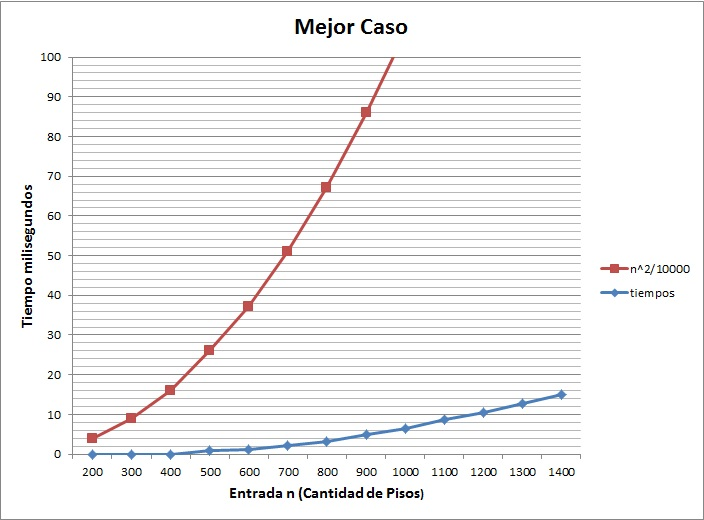
\includegraphics[scale=0.70]{imagenes/MejorCasoEj1.jpg}
	  \end{center}
 \caption{Mejor caso}
\end{figure}

Como la solución mínima de portales, es 1, dado un P fijo, ya que es un portal que va desde el primer hasta el ultimo piso, entonces la solución mas rápida que se puede hacer, es que haya un solo portal, ya que la matriz la vamos a recorrer en $O(n^2)$ y también vamos a agregar 1 portal ($O(n)$).

%\textbf{completar!}

%\newpage

Y nuestro "peor caso", también en base al mismo n fijo, es agregar la máxima cantidad de portales posibles, que es $n*(n-1)/2$, que seria agregar para $i<j<=n$, para cada piso $i=1,2,..,n$ un portal del piso $i$ hasta el piso $j$ con $j=i,i+1,..,n$. Entonces recorreríamos la matriz, en $O(n^2)$ y también la matriz, en $O(n*(n-1)/2)$ que queda en el mismo orden de $O(n^2)$ pero a la hora de la practica se nota una constante que los diferencia. 

\begin{figure}[H]
  \begin{center}
      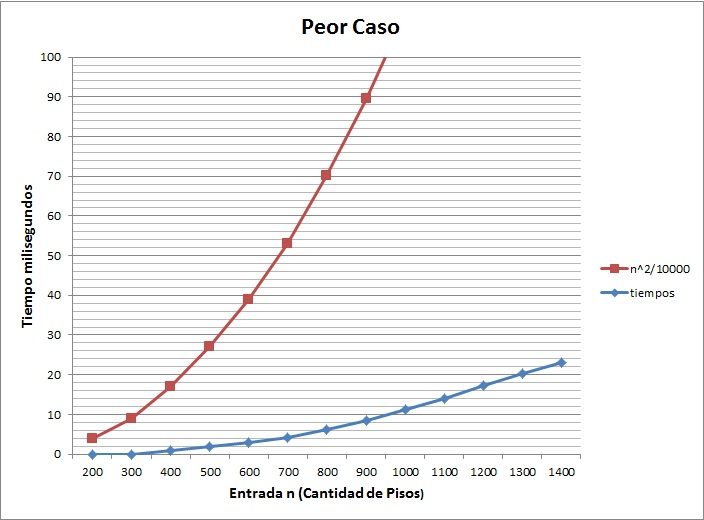
\includegraphics[scale=0.70]{imagenes/PeorCasoEj1.jpg}
	  \end{center}
 \caption{Peor Caso}
\end{figure}



\vspace*{0.3cm}

%\textbf{completar!}




%\newpage

%\vspace*{0.3cm}

%\textbf{completar!}

\begin{figure}[H]
  \begin{center}
      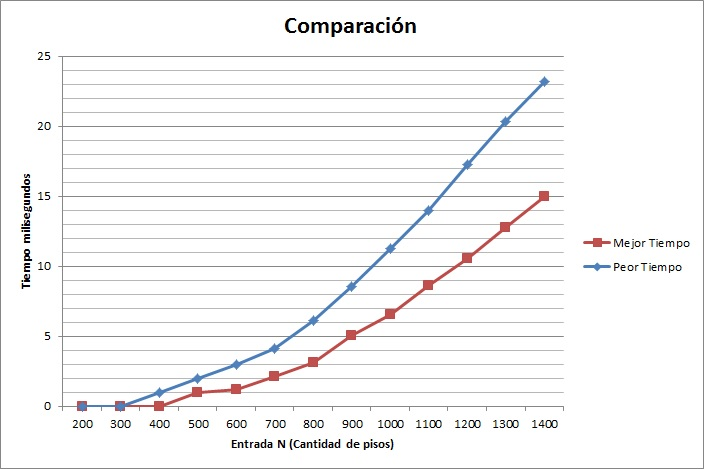
\includegraphics[scale=0.70]{imagenes/ComparacionEj1.jpg}
	  \end{center}
 \caption{Comparación entre el mejor y peor caso}
\end{figure}

Acá brindamos una comparación entre el mejor y  peor caso. aqui podemos notar que las mediciones empíricas de coinciden con lo teórico





%\newpage
%\subsubsection{Test 2}

%\vspace*{0.3cm}

%\textbf{completar!}


%\newpage
%\subsubsection{Test 3}

%\vspace*{0.3cm}

%\textbf{completar!}


\newpage
\section{Problema 2}
\subsection{Descripción del problema.}

\vspace*{0.3cm}
 
%\textbf{Introduccion al problema}
La tecnología avanza a paso agigantados, y nuestro querido pabellón cero+infinito de debe adecuar a la nuevas tecnologías. 
En este caso el pabellón sufre una modificación en su modo de transportar gente de un piso a otro, osea sus portales serán totalmente distintos a como los conocimos ahora. \newline

\begin{figure}[H]
  \begin{center}
      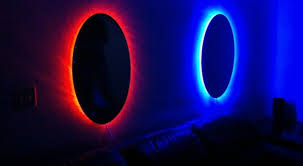
\includegraphics[scale=0.70]{imagenes/portales1.jpeg}
      
\includegraphics[scale=0.70]{imagenes/portales2.jpeg}
  \end{center}
  \caption{Portales del 2048}
  \label{nCte}
\end{figure}

Los cambios que se realizaron son los siguiente: \newline
\begin{itemize}
	\item La cantidad de pisos es N y todos los pasillos miden L unidades de longitud.
	\item Los portales sirven tanto para ascenso como para descenso de un piso a otro piso(tal piso podría ser el mismo).
	\item Los paracaídas quedaron pasado de moda (obsoletos), por lo tanto ya no sera necesario bajar hasta el piso_0  para volver a intentar subir cuando nos equivoquemos.
	\item Como dijimos cada pasillo tiene largo L, dónde a cierta distancia desde origen podrán estar ubicados los portales.
	\item Cada portal nos transportara a otro piso a una cierta distancia del origen del pasillo (tal vez el mismo piso pero a distinta distancia).
	\item Se asegura que en toda instancia del problema es posible realizar el recorrido deseado, y que no hay más de un portal que comunique las mismas posiciones del mismo par de pisos. Observar que puede haber mas de un portal que comuniquen el mismo par de pisos, y portales que comuniquen posiciones diferentes dentro del pasillos de un mismo piso.
	\item El alumno parte siempre del piso_0 y quiere llegar al piso_N donde la puerta del salon esta ubicada al final del pasillo. 
\end{itemize}


 
\textbf{Problema concreto a resolver:} \newline

Todos nuestros estudiantes son muy aplicados, tanto que necesitan llegar de la manera mas rápido(rapidez en tiempo) al aula donde se dicta la materia de  Algoritmos y estructuras de datos III, con lo idea de llenar de consultas a los docentes y presenciar sus clases magistrales. Estos alumnos están muy confundidos con las nuevas funcionalidades de los portales ya descriptos arriba.
El problema consiste en llegar en el menor tiempo posible al aula(piso_N al final del pasillos), osea queremos optimizar el tiempo(en esta caso minimizar tiempo).
Hay que tener cuenta ciertas cosas, para eso voy a dar un poco de notación, condiciones iniciales y finales.
\begin{itemize}
	\item A, $D_A$: B , $D_B$ que indica que el portal $A$ esta Adistancia $D_A$ del pasillo de inicio del piso A, y  te transporta hasta el piso B dónde la salida del portal esta a distancia $D_B$.
	\item Recordar que el alumno siempre comienza desde el piso_0 a distancia cero del pasillo.
	\item Estos alumno tienen como objetivo llegar hasta el piso_N a distancia L, que es justo donde queda la puerta de entrada al salón.
	\item Recorrer 1 metro del pasillo requiere de 1 segundo y utilizar el portal nos demanda 2 segundos(en cualquiera de las dos direcciones). 	 
\end{itemize}
 Damos ejemplo para aclarar como tenemos la entrada y que queremos de salida (input y output).
 Notar que cada portal va estar identificado como una 4-upla  de la siguiente manera $(A,D_A,B,D_B)$. Los valores A, D_A, B y D_B son los mismos que enunciamos mas arriba. 
 \newline
Ejemplo 1:
\begin{figure}[H]
 \begin{center}
     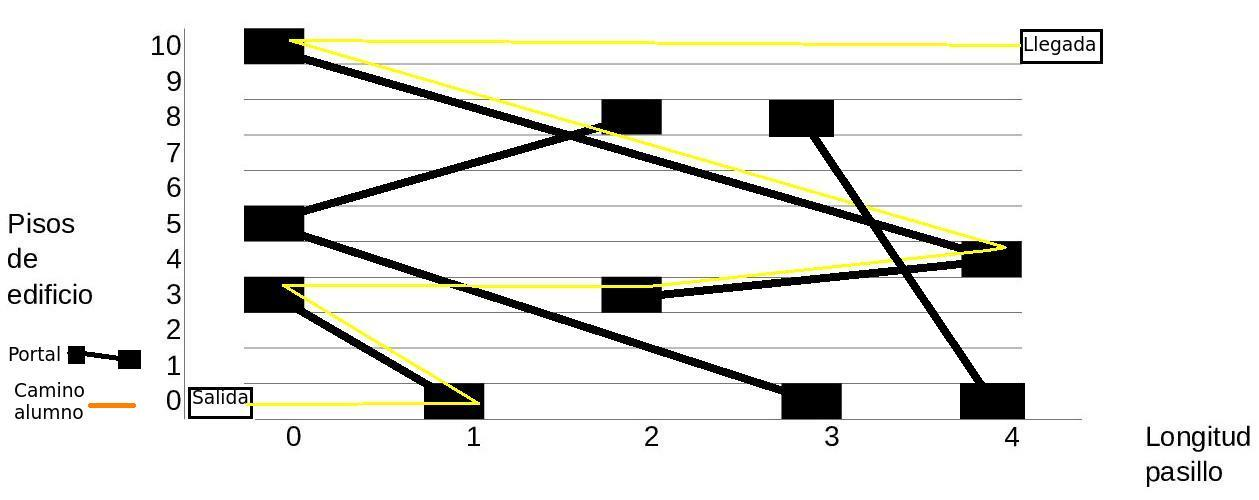
\includegraphics[scale=0.30]{imagenes/ejercicio2ej1.jpg}
 \end{center}
 \caption{ 6 portales, 10 pisos, 4 unidades de longitud de pasillo}
 \label{nCte}
\end{figure}

\begin{itemize}
	\item Entrada : \{ (0,1,3,0),(0,3,5,0)(0,4,8,3)(3,2,4,4)(5,0,8,2)(4,4,10,0)\}
	\item Salida : 13 , que es la cantidad mínima de tiempo que el alumno tarda en llegar al aula(Ver las lineas amarillas del gráfico) 
\end{itemize}

Ejemplo 2: \newline
\begin{figure}[H]
 \begin{center}
     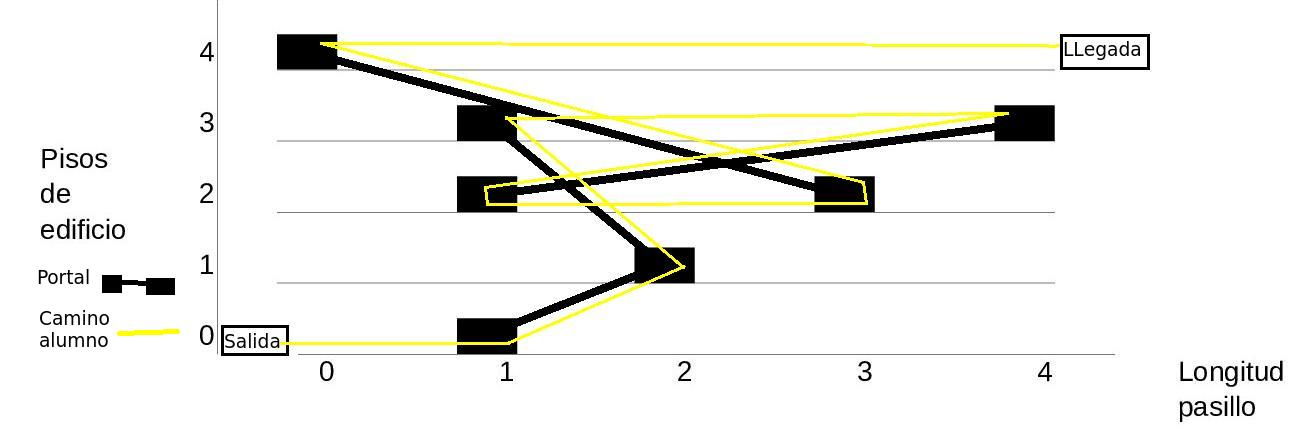
\includegraphics[scale=0.30]{imagenes/ejercicio2ej2.jpg}
 \end{center}
 \caption{ 4 portales, 4 pisos, 4 unidades de longitud de pasillo}
 \label{nCte}
\end{figure}

\begin{itemize}
	\item Entrada : \{ (0,1,2,2),(1,2,3,1),(2,1,3,4),(2,3,4,0)\}
	\item Salida : 18 , que es la cantidad mínima de tiempo que el alumno tarda en llegar al aula(Ver las lineas amarillas del gráfico) 
\end{itemize}
 
%\textbf{completar!}

\subsection{Desarrollo de la idea y pseudocódigo.}

Utilizamos el siguiente procedimiento para obtener la mínima cantidad de segundos necesaria para hacer el recorrido:
Modelamos cada piso de $ L $ metros con $ L+1 $ nodos, y cada portal como un nodo enlazado a los nodos correspondientes según que pisos/metros una. De esta forma podemos considerar que el tiempo que se tarda en ir de un nodo a otro es $1~s$. Para atravesar por un portal hay que pasar por un nodo intermedio, por lo que se gastan $2~s$, en cambio para recorrer un metro, solo $1~s$.

En base a esto implementamos una modificación de $ BFS $, para calcular la distancia entre el nodo correspondiente al metro cero del primer piso, y el correspondiente al último metro del último piso. Para la misma utilizamos una clase especial para los nodos, la cual incluye los atributos $ distancia $ de tipo int, $  marcado$ de tipo bool, $ sucesores $, la cual es una lista de nodos con los sucesores, para la misma consideramos que un nodo es sucesor de otro si están unidos por una arista en el grafo, ya que los portales son bidireccionales, y en los pasillos es posible avanzar y retroceder. Por ultimo los nodos tienen el atributo $ id $ de tipo int, el cual es un número que identifica unívocamente cada nodo. Para los nodos utilizamos los números para identificarlos en orden, es decir, para el primer piso  los números de cero a $ L $, par los del segundo de $ L+1 $ a $ 2L+1 $. y así siguiendo. Para los nodos correspondientes a los portales utilizamos los números siguientes a los ya utilizados para los nodos de los pasillos.

Implementamos en java el algoritmo de $ BFS $ dado en la teórica \cite{teorica}, con la diferencia de que va completando el atributo distancia. Cada vez que se descubre un nuevo nodo se le asigna una distancia de 1 + la distancia de su antecesor, y también se pregunta si su atributo $ id $ es $(N+1)*(L+1)-1)$, en ese caso termina de ejecutar. La solución fue implementada en una clase de java llamada $ Ejercicio2 $.



\subsection{Correctitud}

Para garantizar que nuestro algoritmo es correcto, tiene que valer que el camino que encuentra por primera vez el último nodo, sea el de menor longitud. Esto es verdadero, ya que el algoritmo de $ BFS $, recorre los nodos con distancias en orden, es decir primero los que están a distancia 1, luego los que están a distancia 2, y así siguiendo. Esto se debe a que el algoritmo empieza con un elemento inicial en la cola ''First-in, First-out'', luego encola los sucesores del mismo, los cuales están a distancia uno. Entonces va desencolando de a uno los elementos de la cola y encolando sus sucesores, los cuales están a distancia dos. Como los que primero ingresan son los primeros que salen, primero salen de la cola, los nodos a distancia cero, luego los a distancia uno, dos, y así sucesivamente.


\subsection{Análisis de complejidad}

%\vspace*{0.3cm}

%\textbf{completar!}

Se calcularan las complejidades en base los parámetros de entrada cantidad de portales, denotado por $ P $ , piso mas grande, denotado por $ N $, y cantidad de metros de los pasillos denotado por $ L $.

La complejidad de este algoritmo depende del número de iteraciones antes de encontrar el nodo buscado, para una instancia aleatoria particular, la complejidad dependerá de la configuración de los portales.
El peor caso es cuando se visitan todos los nodos. Analizamos la complejidad en peor caso, en el código del apéndice.  Como en todo algoritmo $bfs$, sobre un grafo, tiene un complejidad en peor caso de $O(n+m)$, donde n es la cantidad de nodos, y m la cantidad de aristas. En este caso tenemos $n=(N+1)*(L+1) +P$, y $m= (N+1)*(L) +2P$, con lo que tenemos una complejidad de $O(N*L+P)$ en peor caso.

El mejor caso es cuando los nodos inicial y final pueden estar conectados por un portal, por lo que la complejidad de la misma será la misma que para elaborar el grafo, la cual es $ O(N*L+P) $ tal como puede verse en el apéndice.


\subsection{Experimentación}

Para generar instancias en peor caso utilizamos la clase $ GenereadorInstanciasEj2 $,el cual al ejecutarse, genera un archivo llamado $ Ej2Instancias.in $ con aquellas. Las mismas consisten en unir los pisos contiguos, por ejemplo el cero con el uno, por medio de portales que comuniquen la baldosa $ L $ de un piso con la cero 
del siguiente. De esta manera para llegar desde el punto de partida al final, se necesitan recorrer todos los metros de todos los pasillos, y pasar por todos los portales, que en este caso tenemos $ P=N $. Si calculamos el resultado esperado en segundos según este recorrido obtenemos: $ Tiempo=(N+1)L+2N $. Se podría demostrar que para esos parámetros de $ N $, $ L $ y $ P $ esa configuración corresponde al peor caso.

Para ese tipo de instancias, se consideraron dos experiencias. En una se deja fijo la cantidad de baldosas $ L $, y se varia la cantidad de pisos, $ N $, con la cual también varia la cantidad de portales $ P $, ya que se mantiene invariante que $ P=N $. En la otra experiencia, se deja fijo $ N $ y $ P $, y se varia $ L $. 

Para tomar tiempos se utilizo la clase $ Ej2Tiempos $, en la cual para cada instancia se corre 600 veces el algoritmo se guardan los resultados en un arreglo. Calculamos el promedio  y el desvío estándar del mismo, y luego lo filtramos quedándonos con los valores que estuvieran entre el promedio menos el desvío estándar y promedio mas el desvío estándar. Finalmente tomamos un promedio de los valores que quedaron, y ese es el resultado que consideramos como tiempo final.

En las figuras~\ref{peorCasoNfijo} y \ref{peorCasoLfijo} podemos ver los resultados obtenidos.

\begin{figure}[H]
\centering
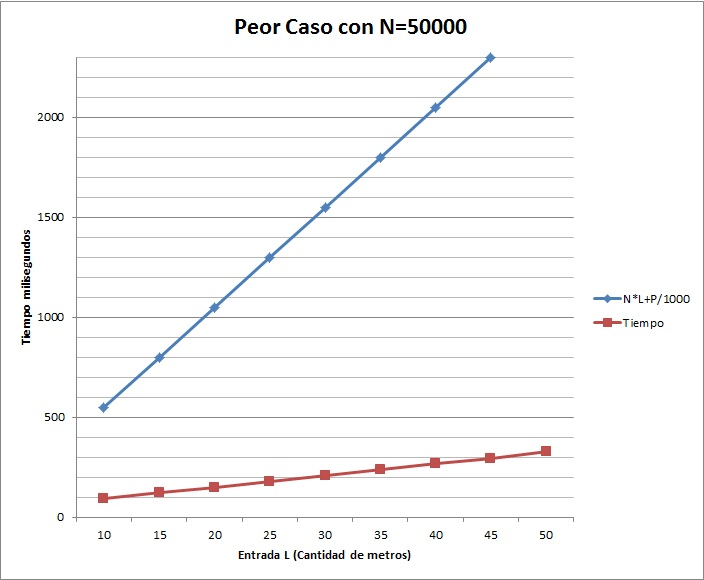
\includegraphics[scale=0.6]{../PeorCasoEj2Nfijo.jpg}
\caption{Gráfico de tiempos obtenidos en función de $L$, para valores de $ N $ y $ P $ fijos en 50000, con una configuración de peor caso para estos tres parámetros.}
\label{peorCasoNfijo}
\end{figure}

En la figura~\ref{peorCasoNfijo} se puede visualizar como el tiempo de computo varia linealmente con $ L $, tal como es de esperarse teóricamente.
\begin{figure}[H]
\centering
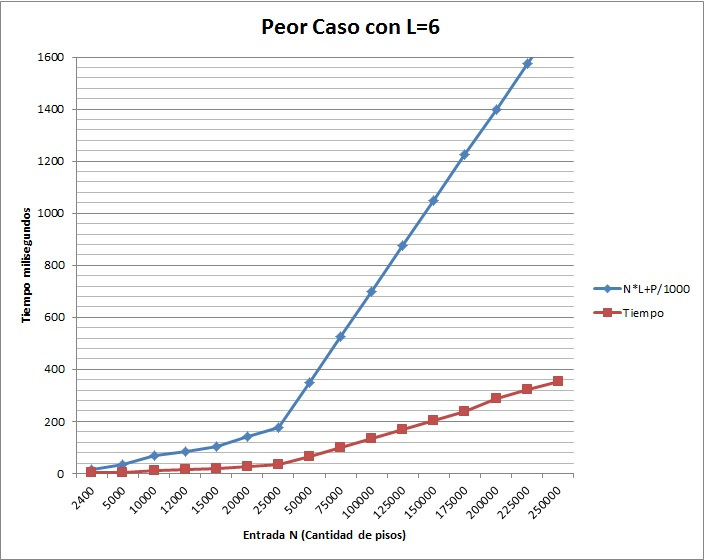
\includegraphics[scale=0.6]{../PeorCasoEj2Lfijo.jpg}
\caption{Gráfico de tiempos obtenidos en función de $N$, para un valor de $ L $  fijo en 6, con una configuración de peor caso para los tres parámetros.}
\label{peorCasoLfijo}
\end{figure}

En la figura~\ref{peorCasoLfijo} se puede visualizar como el tiempo de computo varia según el parámetro $ N $ de la configuración. Podemos distinguir que se comporta en forma similar a la función utilizada para comparar a la misma, la cual se encuentra en la misma figura.

Para el mejor caso se consideraron las instancias ya utilizadas en el peor caso(notar que tienen mismo $ N $, $ L $ y $ P $), pero con la modificación de que el punto inicial con el final estén conectados por un portal, de esta manera el resultado esperado es de dos segundos. Para generar estas instancias utilizamos la clase $ GeneradorInstanciasMejorCaso $, el cual al ejecutarse produce el archivo $ Ej2InstanciasMejorCaso.in $. Nuevamente tomamos tiempos con la clase $ Ej2Tiempos $. En las figuras~\ref{mejorCasoNfijo} y \ref{mejorCasoLfijo} podemos ver los resultados obtenidos.

\begin{figure}[H]
\centering
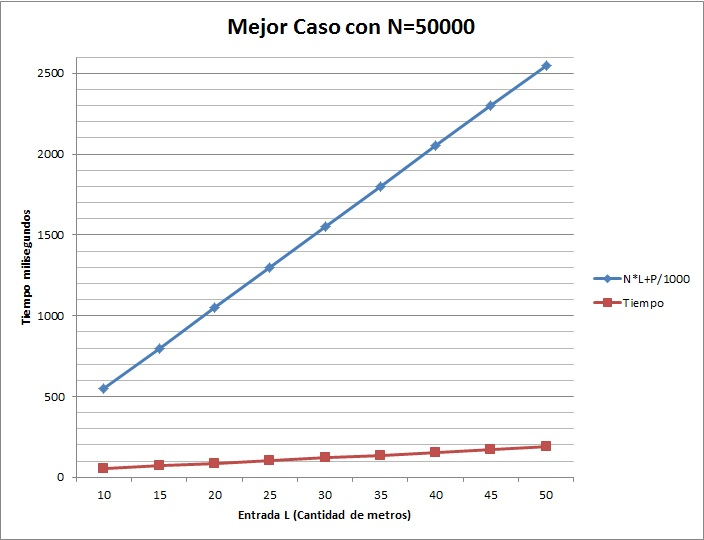
\includegraphics[scale=0.6]{../MejorCasoEj2Nfijo.jpg}
\caption{Gráfico de tiempos obtenidos en función de $L$, para valores de $ N $ y $ P $ fijos en 50000, con una configuración de mejor caso para estos tres parámetros.}
\label{mejorCasoNfijo}
\end{figure}

\begin{figure}[H]
\centering
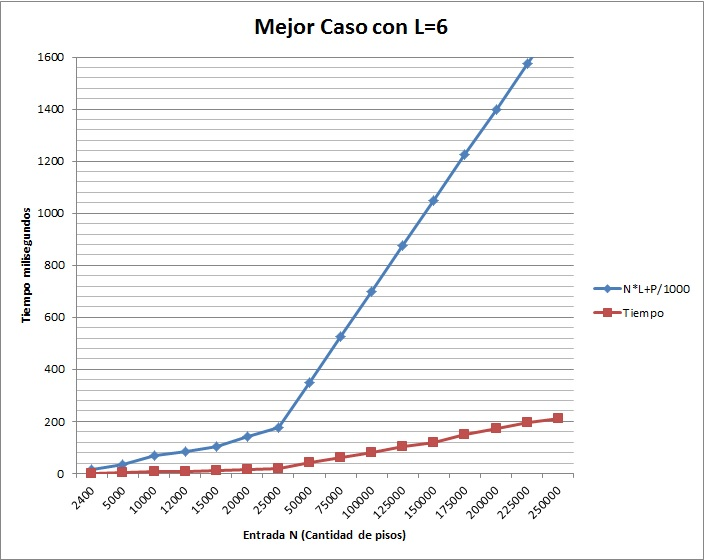
\includegraphics[scale=0.6]{../MejorCasoEj2Lfijo.jpg}
\caption{Gráfico de tiempos obtenidos en función de $N$, para un valor de $ L $  fijo en 6, con una configuración de mejor caso para los tres parámetros.}
\label{mejorCasoLfijo}
\end{figure}

En las figuras~\ref{mejorCasoNfijo} , y \ref{mejorCasoLfijo} podemos ver como el tiempo de computo varia en función de los parámetros para una configuración de mejor caso, en forma análoga a como varia para una de peor caso.

Para el caso aleatorio se generaron instancias con la clase $ GeneradorInstanciasAleatorioMismo $, el cual al ejecutarse las guarda las mismas en $ Ej2InstanciasAleatorioMismo.in $. Se utilizaron los mismos valores de $ N $, $ L $ y $ P $, pero con la particularidad que los pisos y baldosas comunicados se seleccionan aleatoriamente. Se utilizo la clase Random de java con semilla fijada en 55 para generar números aleatorios.

Para constatar que la las instancias aleatorias lleguen al piso deseado, se hizo una modificación de la clase $ Ejercicio2 $, para que en caso de que se encuentre al mismo, imprima por pantalla ''Encontrado'' junto con los valores de $ L $ y $ N $, y así poder identificar si la instancia generada aleatoriamente es valida. En caso de no ser valida, se gasta un $ nextInt $ almacenándolo en una variable extra llamada $ nop $ creada con tal propósito. De esta manera los valores que se obtienen aleatoriamente y se imprimen en el archivo son distintos, obteniendo una nueva instancia(distinta a la que se obtendría sin gastar un $ nextInt $ extra) que posiblemente sea valida. Se repite el procedimiento hasta conseguir que la instancia sea valida, y esto se repite para cada instancia, consiguiendo que todas las instancias generadas sean validas.

En las figuras~\ref{aleatorioCasoNfijo} y \ref{aleatorioCasoLfijo} podemos ver los resultados obtenidos.

\begin{figure}[H]
\centering
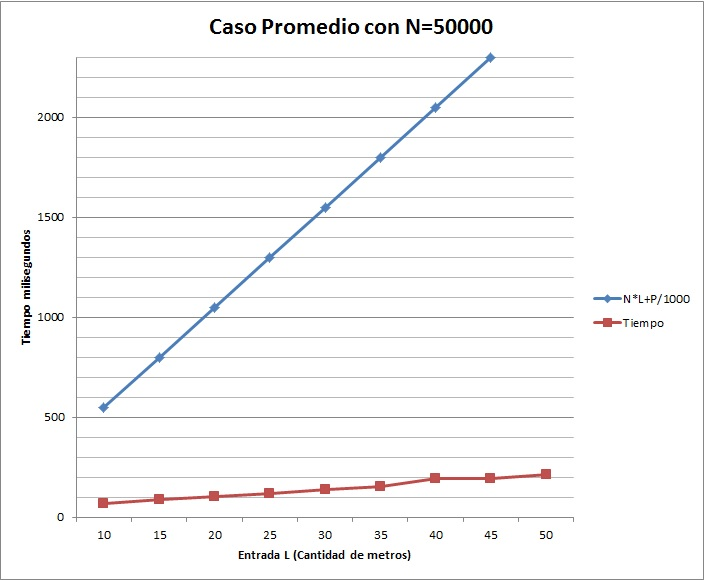
\includegraphics[scale=0.6]{../CasoPromedioEj2Nfijo.jpg}
\caption{Gráfico de tiempos obtenidos en función de $L$, para valores de $ N $ y $ P $ fijos en 50000, con una configuración aleatoria para estos tres parámetros.}
\label{aleatorioCasoNfijo}
\end{figure}

\begin{figure}[H]
\centering
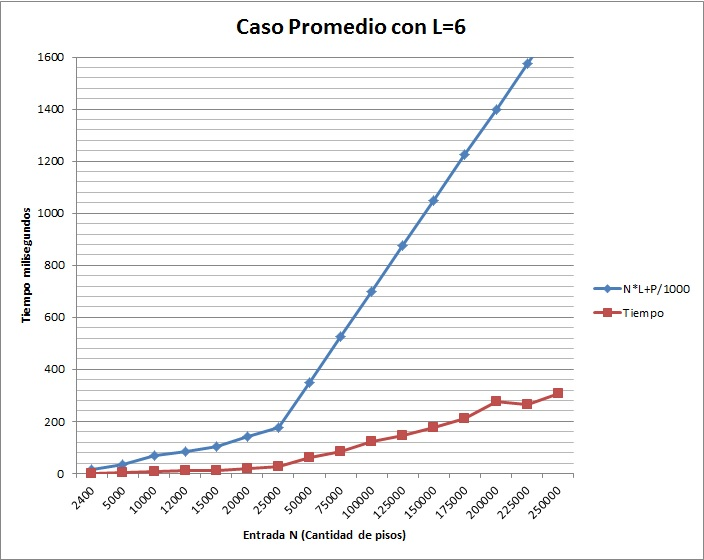
\includegraphics[scale=0.6]{../CasoPromedioEj2Lfijo.jpg}
\caption{Gráfico de tiempos obtenidos en función de $N$, para un valor de $ L $  fijo en 6, con una configuración de mejor caso para los tres parámetros.}
\label{aleatorioCasoLfijo}
\end{figure}

En las figuras~\ref{aleatorioCasoNfijo} y \ref{aleatorioCasoLfijo} podemos distinguir que para configuraciónes aleatorias de $ N $, $ L $ y $ P $, las funciones varían en forma ''similar''' al peor y mejor caso, aunque difieren en no tener un comportamiento tan uniforme.

En cuanto a la comparación entre el tiempo de computo de peor, mejor y caso aleatorio, a pesar de tener el mismo orden de complejidad, en las experiencias se pudo distinguir claramente como las instancias de peor caso tienen un tiempo mayor, seguidas por la de caso aleatorio y por último las de mejor caso. En las figuras \ref{ComparacionCasoNfijo} y \ref{ComparacionCasoLfijo} podemos comparar los tiempos de computo para peor y mejor caso.


\begin{figure}[H]
\centering
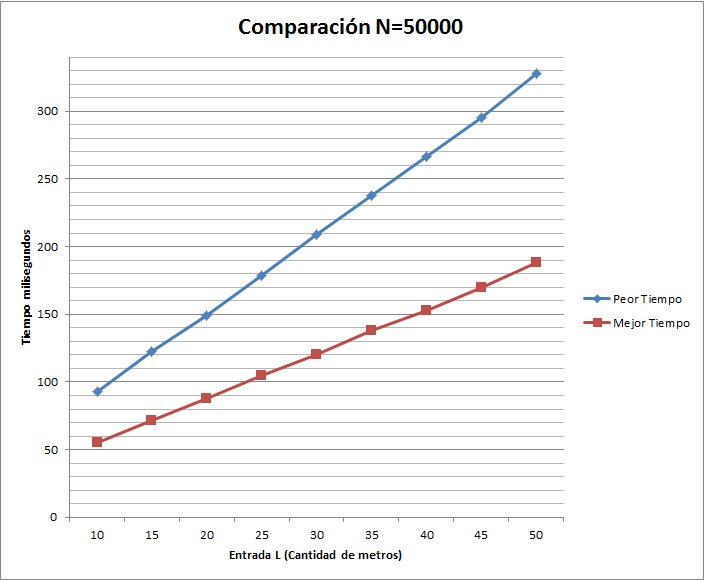
\includegraphics[scale=0.6]{../ComparacionEj2Nfijo.jpg}
\caption{Gráfico de tiempos obtenidos en función de $L$, para valores de $ N $ y $ P $ fijos en 50000, con una configuración de peor y mejor caso para estos tres parámetros.}
\label{ComparacionCasoNfijo}
\end{figure}

\begin{figure}[H]
\centering
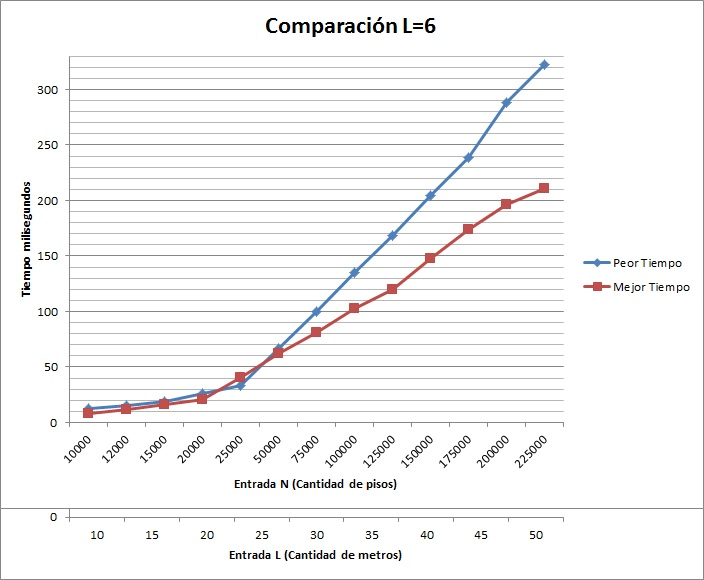
\includegraphics[scale=0.6]{../ComparacionEj2Lfijo.jpg}
\caption{Gráfico de tiempos obtenidos en función de $N$, para un valor de $ L $  fijo en 6, con una configuración de peor y mejor caso. }
\label{ComparacionCasoLfijo}
\end{figure}




\subsection{Validación}

Para validar el algoritmo, utilizamos los casos de test de la cátedra, y también se verificó que el resultado para las instancias de mejor y peor caso utilizadas en la experimentación sea el esperado.

En el archivo $ ResultadosEsperadosPeorCasoEj2.ods $ podemos encontrar los resultados esperados para el peor caso, y para el mejor caso sabemos que tienen que ser todos dos.



\newpage
\section{Problema 3}
\subsection{Descripción del problema.}

\vspace*{0.3cm}

\textbf{Introducción} \newline
En esta época en que el tiempo es muy valioso(''el tiempo es oro''), y no estaría bueno perderlo. Y los alumno del pabellón  cero+infinito no son la excepción. \newline
El edificio fue diseñado con una cantidad de pasillos que podría ser excesivo, y esto traería problemas a los alumno, docentes y comunidad exactas. \newline
 A este problema lo podemos modelar como un grafo ponderado(con pesos en las aristas), donde cada eje es un pasillo y su peso es la longitud del pasillo. Los vértices serian las intersecciones entre pasillos o un extremo dónde termina el dicho pasillo.
En las figuras de abajo vemos un pasillo, el pabellón cero+infinito, y también una muy posible distribución de pasillos de dicho pabellón.  
\begin{figure}[H]
  \begin{center}
      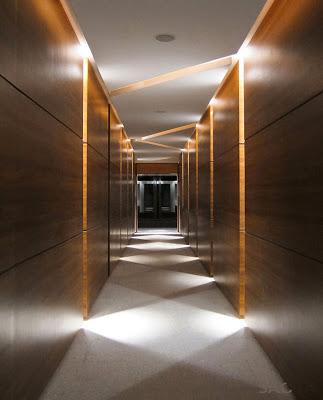
\includegraphics[scale=0.40]{imagenes/pasillo1.jpeg}
      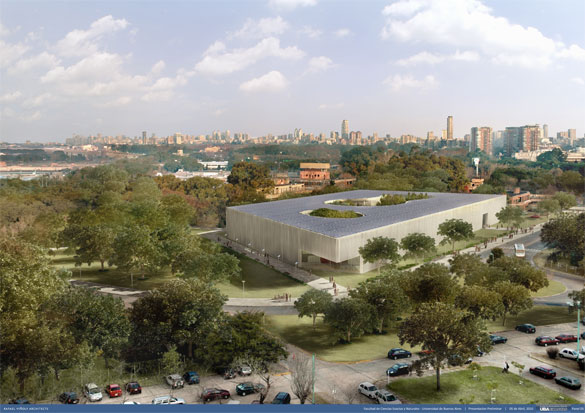
\includegraphics[scale=0.40]{imagenes/cero+infinito1.jpg}
      \caption{Pasillo moderno, pabellón Cero+infinito}
  \end{center}
  \begin{center}    
      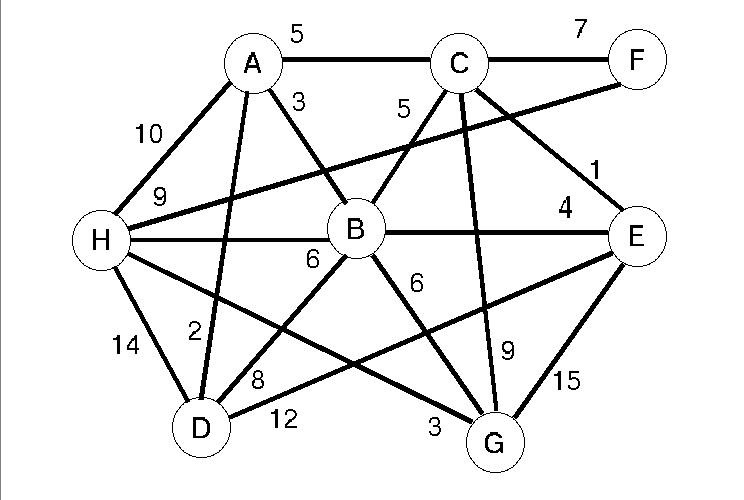
\includegraphics[scale=0.30]{imagenes/grafoPasillo.jpg}
       \caption{Ejemplo de distribución de pasillos del pabellón}
  \end{center}
%  \caption{ejemplo}
\end{figure}

\textbf{Problema} \newline
El decano y el Director del Departamento de Computación, se reunieron para charlar sobre el problema de la mala distribución de los pasillos.
El problemas es que se podrían generar ciclos en el grafo que representa los pasillos, y esto desorientaría a muchos alumnos (peor los alumnos ciclarían infinitamente). Por consiguiente se tomaron medidas para remediar este problema. Se decidió clausurar pasillos de modo tal que queden un grafo sin ciclos. \newline   
Para clausurar hay que tener en cuenta lo siguiente :

\begin{itemize}  
	\item Los pasillos mas largos son más costosos de clausurar.
	\item Debemos devolver la mínima suma de longitudes de pasillos que deben ser clausurados(podría ser ninguno).
	\item La solución la debemos devolver con complejidad $O(M*log(M))$, donde  $M = \# ConjuntoDePasillos$ (cantidad de aristas).
	\item Como precondición tenemos que el grafo es conexo.
\end{itemize}
Como vemos este problema es un caso típico de optimización(en este caso minimización). Acá se quiere minimizar la suma posible de longitudes de pasillos que se quieren clausurar. \newline

En las siguientes lineas vamos a tener conjuntos de 3-uplas que representan las aristas, donde primer y segundo componente son los nodos de incidencia, la tercer componente es el peso de la arista. \newline
  
\textbf{Ejemplos de input y output: } \newline
En las siguientes lineas vamos a tener conjuntos de 3-uplas que representan las aristas, donde primer y segundo componente son los nodos de incidencia, la tercer componente es el peso de la arista.\newline
Ejemplo 1:

\begin{center}
\begin{tikzpicture}[node distance   = 2 cm]
  %\useasboundingbox (-1,-1) rectangle (11,11); 
  \tikzset{VertexStyle/.style = {shape          = circle,
                                 ball color     = orange,
                                 text           = black,
                                 inner sep      = 2pt,
                                 outer sep      = 0pt,
                                 minimum size   = 24 pt}}
  \tikzset{EdgeStyle/.style   = {thick,
                                 double          = orange,
                                 double distance = 1pt}}
  \tikzset{LabelStyle/.style =   {draw,
                                  fill           = yellow,
                                  text           = red}}
     \node[VertexStyle](A){A};
     \node[VertexStyle,right=of A](B){B};
     \node[VertexStyle,right=of B](C){C};
     \tikzset{EdgeStyle/.append style = {bend left}}
     \draw[EdgeStyle](A) to node[LabelStyle]{3} (B);
     \draw[EdgeStyle](B) to node[LabelStyle]{3} (C);
     \draw[EdgeStyle](C) to node[LabelStyle]{3} (A);
  \end{tikzpicture}

\end{center}

\begin{itemize}  
	\item Entrada:  $\{(A,B,3),(B,C,3),(C,A,3) \}$
%	\item Salida: 3, podemos borrar solamente una arista cualquiera (en el dibujo borramos la arista (A,C,3)) para eliminar el ciclo.
\end{itemize}


\begin{center}
\begin{tikzpicture}[node distance   = 2 cm]
  %\useasboundingbox (-1,-1) rectangle (11,11); 
  \tikzset{VertexStyle/.style = {shape          = circle,
                                 ball color     = orange,
                                 text           = black,
                                 inner sep      = 2pt,
                                 outer sep      = 0pt,
                                 minimum size   = 24 pt}}
  \tikzset{EdgeStyle/.style   = {thick,
                                 double          = orange,
                                 double distance = 1pt}}
  \tikzset{LabelStyle/.style =   {draw,
                                  fill           = yellow,
                                  text           = red}}
     \node[VertexStyle](A){A};
     \node[VertexStyle,right=of A](B){B};
     \node[VertexStyle,right=of B](C){C};
     \tikzset{EdgeStyle/.append style = {bend left}}
     \draw[EdgeStyle](A) to node[LabelStyle]{3} (B);
     \draw[EdgeStyle](B) to node[LabelStyle]{3} (C);
  \end{tikzpicture}
\end{center}


\begin{itemize}  
%	\item Entrada:  $\{(A,B,3),(B,C,3),(C,A,3) \}$
	\item Salida: 3, podemos borrar solamente una arista cualquiera (en el dibujo borramos la arista (A,C,3)) para eliminar el ciclo.
\end{itemize}

Ejemplo 2: \newline

\begin{center}
\begin{tikzpicture}[node distance   = 2 cm]
%  \useasboundingbox (-1,-1) rectangle (11,11); 
  \tikzset{VertexStyle/.style = {shape          = circle,
                                 ball color     = orange,
                                 text           = black,
                                 inner sep      = 2pt,
                                 outer sep      = 0pt,
                                 minimum size   = 12 pt}}
  \tikzset{EdgeStyle/.style   = {thick,
                                 double          = orange,
                                 double distance = 2 pt}}
  \tikzset{LabelStyle/.style =   {draw,
                                  fill           = yellow,
                                  text           = red}}
     \node[VertexStyle](A){A};
     \node[VertexStyle,right=of A](B){B};
     \node[VertexStyle,right=of B](C){C};
%     \node[VertexStyle,right=of C](E)(E);
     \node[VertexStyle,above= 4 cm of A](D){D};     
     \node[VertexStyle,above= 4 cm of C](E){E};     

     \draw[EdgeStyle](A) to node[LabelStyle]{8} (B) ;
     \tikzset{EdgeStyle/.append style = {bend left}}
     \draw[EdgeStyle](C) to node[LabelStyle]{10} (D);
     \draw[EdgeStyle](A) to node[LabelStyle]{70} (E);
%     \draw[EdgeStyle](B) to node[LabelStyle]{3} (A);
     \draw[EdgeStyle](A) to node[LabelStyle]{63} (D);
     \draw[EdgeStyle](B) to node[LabelStyle]{53} (C);
     \draw[EdgeStyle](B) to node[LabelStyle]{54} (E);

     \draw[EdgeStyle](E) to node[LabelStyle]{12} (C);
     \draw[EdgeStyle](D) to node[LabelStyle]{22} (E);
  \end{tikzpicture}
\end{center}

\begin{itemize}  
	\item Entrada:  $\{(A,B,8),(A,E,70),(A,D,63),(B,C,53),(B,E,54),(C,D,10),(C,E,12),(D,E,22)\}$
\end{itemize}


\begin{center}
\begin{tikzpicture}[node distance   = 2 cm]
%  \useasboundingbox (-1,-1) rectangle (11,11); 
  \tikzset{VertexStyle/.style = {shape          = circle,
                                 ball color     = orange,
                                 text           = black,
                                 inner sep      = 2pt,
                                 outer sep      = 0pt,
                                 minimum size   = 12 pt}}
  \tikzset{EdgeStyle/.style   = {thick,
                                 double          = orange,
                                 double distance = 2 pt}}
  \tikzset{LabelStyle/.style =   {draw,
                                  fill           = yellow,
                                  text           = red}}
     \node[VertexStyle](A){A};
     \node[VertexStyle,right=of A](B){B};
     \node[VertexStyle,right=of B](C){C};
     \node[VertexStyle,above= 4 cm of A](D){D};     
     \node[VertexStyle,above= 4 cm of C](E){E};     
     \tikzset{EdgeStyle/.append style = {bend left}}
     \draw[EdgeStyle](A) to node[LabelStyle]{70} (E);
     \draw[EdgeStyle](A) to node[LabelStyle]{63} (D);
     \draw[EdgeStyle](B) to node[LabelStyle]{53} (C);
     \draw[EdgeStyle](B) to node[LabelStyle]{54} (E);
  \end{tikzpicture}
\end{center}

\begin{itemize}  
	\item Salida: 52, que es la suma de los pesos mínimos de las aristas que debo borrar (52 = 8+10+12+22), para sacar los ciclos de este grafo.
\end{itemize}

Observar que en los dos ejemplos anteriores encontramos el árbol generador máximo.
%\begin{itemize}
	%\item Entrada:  $\{(A,B,3),(B,C,3),(C,A,3) /}$ 
	%\item Salida: 3
%\end{itemize}	


%\begin{center}
%\begin{tikzpicture}[node distance   = 4 cm]
%  \useasboundingbox (-1,-1) rectangle (11,11); 
%  \tikzset{VertexStyle/.style = {shape          = circle,
%                                 ball color     = orange,
%                                 text           = black,
%                                 inner sep      = 2pt,
%                                 outer sep      = 0pt,
%                                 minimum size   = 24 pt}}
%  \tikzset{EdgeStyle/.style   = {thick,
%                                 double          = orange,
%                                 double distance = 1pt}}
%  \tikzset{LabelStyle/.style =   {draw,
%                                  fill           = yellow,
%                                  text           = red}}
%     \node[VertexStyle](A){A};
%     \node[VertexStyle,right=of A](B){B};
%     \node[VertexStyle,right=of B](C){C};
%     \node[VertexStyle,above= 8 cm of B](D){D};     
%     \draw[EdgeStyle](B) to node[LabelStyle]{1} (D) ;
%     \tikzset{EdgeStyle/.append style = {bend left}}
%     \draw[EdgeStyle](A) to node[LabelStyle]{2} (B);
%     \draw[EdgeStyle](B) to node[LabelStyle]{3} (A);
 %    \draw[EdgeStyle](B) to node[LabelStyle]{4} (C);
%     \draw[EdgeStyle](C) to node[LabelStyle]{5} (B);
%     \draw[EdgeStyle](A) to node[LabelStyle]{6} (D);
%     \draw[EdgeStyle](D) to node[LabelStyle]{7} (C);

%  \end{tikzpicture}
%\end{center}
%\end{document}

%\begin{figure}[htb]
%  \begin{center}
%      \includegraphics[scale=0.25]{imagenes/ejemplo.jpg}
%  \end{center}
%  \caption{ejemplo}
%\end{figure}


\subsection{Desarrollo de la idea y pseudocódigo.}

\vspace*{0.3cm}


Vamos a crear un árbol generador máximo del grafo de pasillos, para así quedarnos con los ejes más chicos que forman un ciclo. La suma de estos ejes es el costo mínimo a pagar para eliminar los ciclos en el grafo.
Para que este problema nos de en orden O($m*log(m)$), siendo m la cantidad de pasillos, utilizaremos la representación en lista de adyacencia del grafo de pasillos. Para generar el árbol generador máximo usaremos un algoritmo muy parecido de Kruskal junto con UnionFind, para que nos de en complejidad pedida. La diferencia entre Kruskal y nuestro algoritmo es que este en vez de agarrar primero las aristas más chicas, tomará las aristas más grande, formado el árbol generador máximo.

\textbf{pseudocodigo} %\newline 

\begin{codebox}
\Procname{$\proc{solve}(int \ n, vector<Aristas> \& portales)	$}
	\li \Comment inicializo $conj$, como un conj vacio y $peso$ en cero
	\li $Ordenar(portales)$	
	\li \Comment Ordeno de mayor a menor segun la longitud del pasillo
	\li \For $i \gets 0$ \To $portales.size$ \Do
	\li		\If generaCiclos($portales[i]$)
	\li			\Then $peso $=$ peso $+$ portales[i].longitud$
	\li 				\Else agregar($conj, portales[i]$) 
			\End
		\End
	\li \Return $peso$
\end{codebox}


\subsection{Justificación de la resolución y demostración de correctitud.}

\vspace*{0.3cm}

%\textbf{completar!}
Ahora probaremos que el algoritmo prepuesto resuelve el problema. Lo que se quiere es eliminar los ciclos con el menor costo. El eliminar los ciclos nos deja un árbol generador del grafo de pasillos, ya que queda un grafo acíclico y conexo. Si el grafo que queda no es conexo significa que habríamos sacado una arista que era el único camino posible entre, por lo menos, un par de nodos, lo que dice que esa arista no era parte de un ciclo. Entonces una solución con esa arista nos daría un costo menor. \newline 
Ahora, como queremos un árbol generador que deje afuera la aristas menos pesadas, para conseguir un costo mínimo, tenemos que generar un árbol que contenga las aristas mas pesadas de los ciclo del grafo, para que queden fuera de este la más livianas. Esto lo hacemos de la misma manera en que el algoritmo de Kruskal genera un AGM, en cada paso agregamos la arista con el peso máximo que no genera ciclos, por lo que nos queda un árbol generador máximo. Por lo tanto, las aristas que quedaron fuera de ese árbol son las aristas más livianas que, al agregarlas, forman un ciclo en el grafo, así que sumadas dan el costo mínimo para eliminar los ciclos.

\subsection{Análisis de complejidad.}

\vspace*{0.3cm}

%\textbf{completar!}
La complejidad de este algoritmo es O($m*log(m)$) siendo m la cantidad de pasillos, ya que esto es lo que tarda realizar el Kruskal modificado.\newline
 El Kruskal modificado tiene complejidad O($m*log(m)$) ya que su  operación más costosa, y la primera en realizarse, es ordenar las aristas y esto lo hace en O($m*log(m)$) ya que sort de \verb-C++- tarda O($n*log(n)$)(según la biblioteca standar de \verb-C++-), siendo n la cantidad de elementos en la lista. Como sort ordena de menor a mayor, lo siguiente en hacerse es usar la instrucción reverse de \verb-C++- que tiene O$\left(\displaystyle\frac{n}{2}\right)$(según biblioteca estándar de \verb-C++-) y la vuelta los valores del vector. Después realizamos la operación de crear un UnionFind para los vértices que tiene O($v$), siendo v la cantidad de vértices, pero $m>=v-1$, por ser un grafo conexo, por lo que es O($m$). Por último, realizamos un for donde todas las operaciones dentro de él son O($1$) o son, Union, para que los dos vértices de la arista agregada a el árbol estén en el mismo conjunto, o isSameSet, para verificar que los extremos de la arista no estén en el mismo conjunto ya que si es así, entonces al agregarla se generaría un ciclo. Entonces, como vimos en clase, si hay una secuencia de m operaciones de makeSet, findSet, unionSet, estas se vuelve orden constante, lo que deja a todos las operaciones del for en O($m$)\newline
 Este algoritmo, con cantidad de vértices(v) y aristas(m) constantes, no tiene un mejor o peor caso, ya que se tienen que recorrer siempre todas las aristas. Se puede hablar de un mejor o peor caso según la cantidad de vértices del grafo, ya que teniendo una cantidad v de vértices uno puede tener más o menos aristas. Entonces podemos hablar de un peor caso el grafo es completo, ya que es la máxima cantidad$\left(\displaystyle\frac{v*(v-1)}{2}\right)$ de aristas que podría tener dado un v. Y de un mejor caso cuando el grafo ya sea un árbol($v-1$), es decir no tiene ciclos, ya que es la menor cantidad de aristas que puede tener un grafo conexo dado un v. Suponiendo que sort de c verifica si la lista esta ordenada y que esto lo hace en orden lineal podemos hacer que nuestro mejor caso deje las aristas ordenadas de menor a mayor, esto generaría que su complejidad sea O($m$) en vez de O($m*log(m)$).

\subsection{Experimentación y gráficos.}

Par las instancias de toma de tiempos del problema 3 lo que hacemos es, si queremos un mejor caso, desde 1 hasta v, siendo v la cantidad de vértices, creamos una arista de el vértice actual al siguiente con peso igual al vértice, para así generar un árbol, y que las aristas estén ordenadas por su peso. Si lo que buscamos es un peor caso, desde 1 hasta v, creamos aristas que van desde el vértice actual hasta todos los siguientes con un peso random, así generamos un grafo completo. Esto se puede realizar por $instanciasEj3.cpp$, pero al utilizarlo nos dimos cuanta que las instancias podían ser muy grandes y pesadas. Por lo cual decidimos hacer que el mismo $TP2EJ3.cpp$ genere cada instancia y tome los tiempos, esto se hace pasando como parámetro un 2.\newline
Para tomar los tiempos corremos 100 veces cada instancia y tomamos el promedio de los resultados que estén entre el promedio más la desvío estándar y el promedio menos el desvío estándar. Este desvío lo calculamos realizando la raíz cuadrada de la varianza, que se puede calcular restándole a cada uno de los tiempos el promedio, elevándolos al cuadrado y después se saca el promedio de todos esos.
\newline\newline
En los siguientes gráficos tenemos los resultados obtenidos...

\begin{figure}[H]
  \begin{center}
      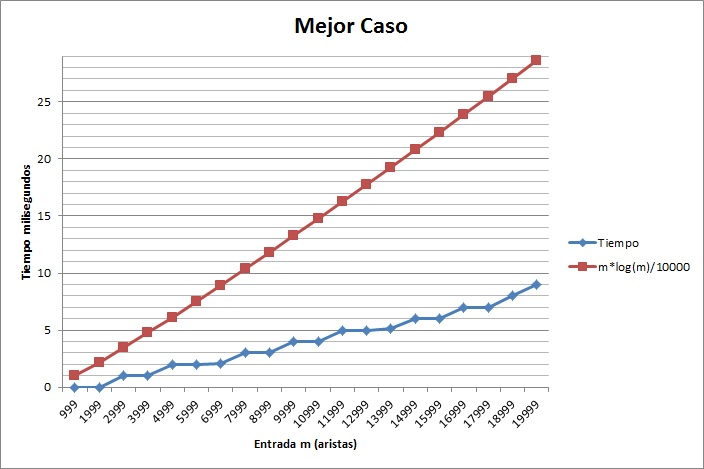
\includegraphics[scale=0.70]{../MejorCasoEj3.jpg}
  \end{center}
 \end{figure}

Este gráfico muestra como el mejor caso de nuestro algoritmo esta siempre acotado por la curva $m*log(m)$. También muestra que a medida que hay más cantidad de vértices la curva con nuestros tiempos se aleja de la curva $m*log(m)$ lo que permite suponer con mayor certeza que el sort de c tarda menos si las aristas ya están ordenadas. Este gráfico apoya nuestra demostración de complejidad, aunque no lo comprueba, porque este caso siempre va a tener mejor tiempo que los otros.

\begin{figure}[H]
  \begin{center}
      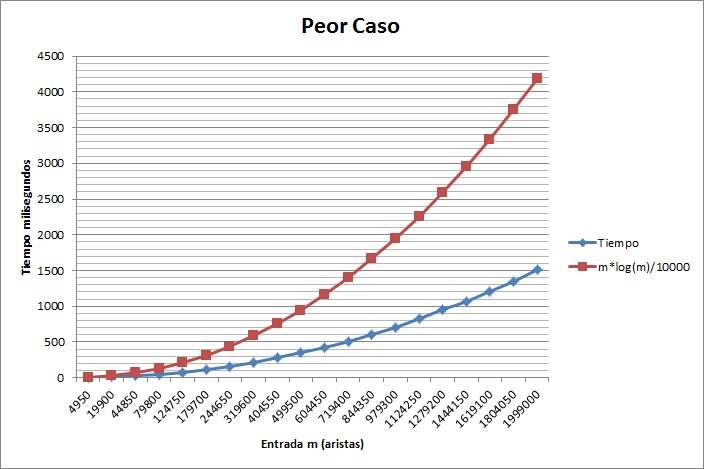
\includegraphics[scale=0.70]{../PeorCasoEj3.jpg}
  \end{center}
 \end{figure}

Este segundo gráfico permite corroborar con más certeza que el anterior la cota en nuestra complejidad, ya que muestra como una curva $m*log(m)$ acota todos los tiempos tomados para el peor caso y, además, se puede observar que nuestros tiempos forman una curva similar a la de $m*log(m)$. También se puede ver como estas dos curvas se van alejando a medida que aumenta la cantidad de vértices.

\subsection{Validación}

Para validar el algoritmo, utilizamos casos de test, los cuales son una expansión de los test de la cátedra, para los cuales conocemos cual es la salida. Las instancia para validar se encuentran en $Tp2Ej3.in$ y las salidas correspondientes a esas instancias se encuentran en $Tp2Ej3.out$. Corriendo $TP2EJ3.cpp$ con los parámetros 1 y $Tp2Ej3.in$ se obtienen los resultados de nuestro algoritmo para esas instancias, estas se guardan en el archivo $TP2Ej3nuestro.out$. Se pueden comparar ambas archivos corriendo $testCorrectitud.cpp$ pasando como parámetro las dos salidas.

%\section{Apéndice 1: Secciones relevantes del código}


\subsection{Código del Problema 2}

\begin{lstlisting}

		FileInputStream entrada =null;  
		BufferedReader reader =null;
		FileWriter escribidor=null;
		
		try{
			entrada = new FileInputStream(args[0]);
			reader = new BufferedReader(new InputStreamReader(entrada));
			escribidor= new FileWriter("Ej2.out");				
			String line=null;	
			int L;
			int N;	
			String[] LyN;
			String[] portales;
			Nodo[] nodosGrafo;	
			while(true){
				
				line=reader.readLine();
				if (line==null) break;

				LyN=line.split(" ");
				L=Integer.parseInt(LyN[0]);
				N=Integer.parseInt(LyN[1]);
				
				line=reader.readLine();
				portales=line.split(";");
				
				nodosGrafo= new Nodo[(L+1)*(N+1)+portales.length];// almacenamos en este arreglo los nodos correspondiendose el indice con el id del nodo
				
				//creamos los nodos
				for(int i=0;i<(L+1)*(N+1);i++){ //complejidad del ciclo O(N*L)
					Nodo nuevo=new Nodo(i);
					nodosGrafo[i]=nuevo;
				}
				
				//asignamos los sucesores de los nodos
				for(int i=0;i<(L+1)*(N+1);i++){  //complejidad del ciclo O(N*L)
					if(i%(L+1)==0) nodosGrafo[i].addSucesor(nodosGrafo[i+1]);
					else if(i%(L+1)==L) nodosGrafo[i].addSucesor(nodosGrafo[i-1]);
					else{
						nodosGrafo[i].addSucesor(nodosGrafo[i+1]);
						nodosGrafo[i].addSucesor(nodosGrafo[i-1]);
					}
				}
				
				//asignamos los sucesores de los portales
				int pisoDesde;
				int baldosaDesde;
				int pisoHasta;
				int baldosaHasta;
				String[] parametrosPortales;
				for(int i=0;i<portales.length;i++){//complejidad del ciclo O(P)
					int idp=(L+1)*(N+1)+i;
					Nodo nodoPortal=new Nodo(idp);
					nodosGrafo[idp] =nodoPortal;
					parametrosPortales=portales[i].trim().split(" ");
				//	System.out.println(parametrosPortales);
					
					pisoDesde=Integer.parseInt(parametrosPortales[0]);
					baldosaDesde=Integer.parseInt(parametrosPortales[1]);
					pisoHasta=Integer.parseInt(parametrosPortales[2]);
					baldosaHasta=Integer.parseInt(parametrosPortales[3]);

					nodoPortal.addSucesor(nodosGrafo[pisoDesde*(L+1)+baldosaDesde]);
					nodosGrafo[pisoDesde*(L+1)+baldosaDesde].addSucesor(nodoPortal);
					
					nodoPortal.addSucesor(nodosGrafo[pisoHasta*(L+1)+baldosaHasta]);
					nodosGrafo[pisoHasta*(L+1)+baldosaHasta].addSucesor(nodoPortal);
				}
				
				//tenemos una complejidad de O(N*L+P) antes de aplicar bfs
				
				//aplicamos bfs
				
				Queue<Nodo> cola= new LinkedList<Nodo>();
				cola.add(nodosGrafo[0]);
				nodosGrafo[0].marcar();
				bfs:
				while(!(cola.isEmpty())){
					Nodo w=cola.remove();
					for(Nodo z : w.getSucesores()){ //complejidad O(d(w)) (donde d(w) indica la cantidad de sucesores de w)
						if(z.getId()==(N+1)*(L+1)-1){
							System.out.println(w.getDistancia()+1);
							escribidor.write(Integer.toString(w.getDistancia()+1));						
							escribidor.write("\n");
							break bfs;
						}	
						if(!(z.isMarcado())){
							z.marcar();
							cola.add(z);
							z.setDistancia(w.getDistancia()+1);
						}
					}
				}// la complejidad de este ciclo depende de el numero de iteraciones antes de encontrar el nodo buscado, en el peor caso se visitan todos los nodos


\end{lstlisting}
\section{}
\begin{thebibliography}{abbrvnat}
\bibitem{teorica} Teórica de Algoritmos y Estructuras de datos III, Departamento Computación, Facultad de Ciencias Exactas y Naturales, UBA.
\end{thebibliography}


\newpage
\section{Informe de modificaciones}

En esta sección se enumeraran las modificaciones que se le hicieron al informe ejercicio por ejercicio.

Ejercicio 1: \newline

1) Se modifico la subsección de \underline{descripción del problema} dado que estaba mal redactado.

2) Se modifico la subsección de \underline{desarrollo de la idea y pseudocódigo} de la siguiente manera:
	\begin{itemize}
		\item Se agrego pseudocódigo.
		\item Se volvió a explicar el desarrollo de la idea de modo que quede mas clara la resolución del problema y se agregaron referencias a fragmentos del pseudocódigo de tal forma que sea mas amena la lectura.
	\end{itemize}
	
3) Se modifico la subsección de \underline{justificación de la resolución y demostración de correctitud}.	
	
4) Se modifico la subsección de \underline{Análisis de complejidad propuesta} de la siguiente manera:	
	\begin{itemize}
		\item Se modifico la explicación de la complejidad propuesta, de manera tal que quede en forma ordenada.
		\item Se agregaron referencias al pseudocódigo, para que el entendimiento de la complejidad se mas legible.
	\end{itemize}

Ejercicio 2: \newline

1) Se agrego una cita.

\bigskip

Ejercicio 3: \newline

1) Se modifico la subsección de \underline{desarrollo de la idea y pseudocódigo} agregando el pseudocódigo.

2) Se modifico la subsección de \underline{Análisis de complejidad.} explicando para que se utiliza el Union Find

3) Se modifico la subsección de \underline{Experimentación y gráficos.} cambiando los gráficos.

\newpage
\section{Apéndice 1: Secciones relevantes del código}
En esta sección, adjuntamos parte del código correspondiente a la resolución de cada problema
que consideramos más relevante.

\subsection{Código del Problema 1}

\begin{lstlisting}[style=customc]
#include<iostream>
#include<cassert>
#include<vector>

using namespace std;

struct Portal{
    int pisoDesde,pisoHasta;
};

class Ejercicio1{
public:
    int solve(int n, vector<Portal> &portales)
    {
		//Primero deberia leer los portales e ir agregando a la matriz los portales..
		//El problema esta resuelto con programacion dinamica, la forma bottom up, primero empezaremos llenandola con los datos que tenemos.
		//Y luego recorriendola, de forma diagonal, y ya sabiendo que cualquier dato que necesitamos ya lo tenemos precalculado.
		int matriz[n][n];
		
		//La lleno con 0, ya que si tiene un 0 quiere decir que no puede llegar, y luego vamos a leer los portales..
		int i=0,j=0;
		for(i = 0; i < n;i++){
			for(j = 0;j < n; j++){
				matriz[i][j] = 0;
			}
		}
		int pisoD,pisoH,suma;
		Portal p1;
		
		//En este for ingreso los portales..
		for(i =0;i< portales.size();i++){
			p1 = portales[i];
			pisoD = p1.pisoDesde;
			pisoH = p1.pisoHasta;
			matriz[pisoD-1][pisoH-1] = 1;
		}
		//Ahora vamos a empezar a recorrer de forma diagonal
		for(i = 1;i<n;i++){ //Voy a hacer este for n veces, lo de adentro del for es del orden: O(n-i+i) => O(n) => O(n*n)
			int max = 0;
			for(j =0;j<i;j++){ //Voy a hacer este for i veces, y lo de adentro es del orden de O(1) => tarda O(i)
				if(matriz[j][i] > max){
					max = matriz[j][i];
				}
			}
			//Tengo el maximo de mi columna, lo que quiere decir que es lo que tardo en llegar hasta mi piso.
			matriz[i][i] = max;
			for(j = i+1;j<n;j++){ //Este for va a iterar n-i veces y lo de adentro lo hace en O(1) => tarda O(n-i)
				if(max == 0){
					matriz[i][j] = 0;
				}else{
					//Tengo que sumarle lo que tardo en llegar a mi piso, si es que ese piso (m [i][j] es accesible, osea tiene un 1)
					if(matriz[i][j] != 0){
						matriz[i][j] = max +1;
					}
				}
			}
		}

		return matriz[n-1][n-1];
    }
};
\end{lstlisting}


\subsection{Código del Problema 2}

\begin{lstlisting}

		FileInputStream entrada =null;  
		BufferedReader reader =null;
		FileWriter escribidor=null;
		
		try{
			entrada = new FileInputStream(args[0]);
			reader = new BufferedReader(new InputStreamReader(entrada));
			escribidor= new FileWriter("Ej2.out");				
			String line=null;	
			int L;
			int N;	
			String[] LyN;
			String[] portales;
			Nodo[] nodosGrafo;	
			while(true){
				
				line=reader.readLine();
				if (line==null) break;

				LyN=line.split(" ");
				L=Integer.parseInt(LyN[0]);
				N=Integer.parseInt(LyN[1]);
				
				line=reader.readLine();
				portales=line.split(";");
				
				nodosGrafo= new Nodo[(L+1)*(N+1)+portales.length];// almacenamos en este arreglo los nodos correspondiendose el indice con el id del nodo
				
				//creamos los nodos
				for(int i=0;i<(L+1)*(N+1);i++){ //complejidad del ciclo O(N*L)
					Nodo nuevo=new Nodo(i);
					nodosGrafo[i]=nuevo;
				}
				
				//asignamos los sucesores de los nodos
				for(int i=0;i<(L+1)*(N+1);i++){  //complejidad del ciclo O(N*L)
					if(i%(L+1)==0) nodosGrafo[i].addSucesor(nodosGrafo[i+1]);
					else if(i%(L+1)==L) nodosGrafo[i].addSucesor(nodosGrafo[i-1]);
					else{
						nodosGrafo[i].addSucesor(nodosGrafo[i+1]);
						nodosGrafo[i].addSucesor(nodosGrafo[i-1]);
					}
				}
				
				//asignamos los sucesores de los portales
				int pisoDesde;
				int baldosaDesde;
				int pisoHasta;
				int baldosaHasta;
				String[] parametrosPortales;
				for(int i=0;i<portales.length;i++){//complejidad del ciclo O(P)
					int idp=(L+1)*(N+1)+i;
					Nodo nodoPortal=new Nodo(idp);
					nodosGrafo[idp] =nodoPortal;
					parametrosPortales=portales[i].trim().split(" ");
				//	System.out.println(parametrosPortales);
					
					pisoDesde=Integer.parseInt(parametrosPortales[0]);
					baldosaDesde=Integer.parseInt(parametrosPortales[1]);
					pisoHasta=Integer.parseInt(parametrosPortales[2]);
					baldosaHasta=Integer.parseInt(parametrosPortales[3]);

					nodoPortal.addSucesor(nodosGrafo[pisoDesde*(L+1)+baldosaDesde]);
					nodosGrafo[pisoDesde*(L+1)+baldosaDesde].addSucesor(nodoPortal);
					
					nodoPortal.addSucesor(nodosGrafo[pisoHasta*(L+1)+baldosaHasta]);
					nodosGrafo[pisoHasta*(L+1)+baldosaHasta].addSucesor(nodoPortal);
				}
				
				//tenemos una complejidad de O(N*L+P) antes de aplicar bfs
				
				//aplicamos bfs
				
				Queue<Nodo> cola= new LinkedList<Nodo>();
				cola.add(nodosGrafo[0]);
				nodosGrafo[0].marcar();
				bfs:
				while(!(cola.isEmpty())){
					Nodo w=cola.remove();
					for(Nodo z : w.getSucesores()){ //complejidad O(d(w)) (donde d(w) indica la cantidad de sucesores de w)
						if(z.getId()==(N+1)*(L+1)-1){
							System.out.println(w.getDistancia()+1);
							escribidor.write(Integer.toString(w.getDistancia()+1));						
							escribidor.write("\n");
							break bfs;
						}	
						if(!(z.isMarcado())){
							z.marcar();
							cola.add(z);
							z.setDistancia(w.getDistancia()+1);
						}
					}
				}// la complejidad de este ciclo depende de el numero de iteraciones antes de encontrar el nodo buscado, en el peor caso se visitan todos los nodos


\end{lstlisting}

\subsection{Código del Problema 3}

\begin{lstlisting}[style=customc]

class Arista{
	private:
		unsigned int _nod1, _nod2;
		int _peso;
		
	public:
		Arista(unsigned int n1, unsigned int n2, int p) : _nod1(n1), _nod2(n2), _peso(p) {}
		int peso() const { return _peso; }
		unsigned int nodo1() const { return _nod1; }
		unsigned int nodo2() const { return _nod2; }
		
		bool operator<(const Arista &ar) const {
			if(peso() != ar.peso()) return peso() < ar.peso();
			if(nodo1() != ar.nodo1()) return nodo1() < ar.nodo1();
			return nodo2() < ar.nodo2();
		}

};

class UnionFind{
	private:
		vector<unsigned int> _parent, _rank;
		
	public:
		UnionFind(unsigned int n){
			for(unsigned int i = 0; i < n; i++){
				_parent.push_back(i);
				_rank.push_back(0);
			}
		}
		
		unsigned int findSet(unsigned int i){ 
			if(_parent[i] == i){
				return i;
			}else{
				_parent[i] = findSet(_parent[i]);
				return _parent[i];
			}
		}
		
		bool isSameSet(unsigned int i, unsigned int j){
			return findSet(i) == findSet(j);
			
		}
		
		void unionSet(unsigned int i, unsigned int j){
			if( !isSameSet(i,j) ){
				unsigned int jParent = findSet(j);
				unsigned int iParent = findSet(i);
				if(_rank[iParent] > _rank[jParent]){
					_parent[jParent] = iParent;
				}else if(_rank[iParent] < _rank[jParent]){
					_parent[iParent] = jParent;
				}else{
					_parent[jParent] = iParent;
					_rank[iParent]++; 
				}
			}
		}
};

int kruskalModificado(int n, vector<Arista> todas){
	sort(todas.begin(), todas.end());
	reverse(todas.begin(), todas.end());
	UnionFind arbol = UnionFind(n);
	int peso = 0;
	for(unsigned int i = 0; i < todas.size(); i++){
		if( !arbol.isSameSet(todas[i].nodo1(), todas[i].nodo2()) ){
			arbol.unionSet(todas[i].nodo1(), todas[i].nodo2());
		}else{
			peso = peso + todas[i].peso();
		}
	}
	return peso;
}

\end{lstlisting}




%\vspace*{0.5cm}

%\begin{lstlisting}
%int main(){
%  return 0;
%}
%\end{lstlisting}


%\vspace*{0.5cm}

%\newpage
%\subsection{Código del Problema 3}

%\begin{lstlisting}
%int main(){
%  return 0;
%}
%\end{lstlisting}

%\vspace*{0.5cm}

%\begin{lstlisting}
%int main(){
%  return 0;
%}
%\end{lstlisting}




\end{document}
